\documentclass[preprint]{JHEP3} % 10pt is ignored!

\JHEPspecialurl{http://jhep.sissa.it/JOURNAL/JHEP3.tar.gz}
\usepackage{graphicx}
\usepackage{amsmath,amssymb}
\usepackage{cite}
\usepackage{multirow}

%\newcommand{\DF1A}{\Delta F_{1,A}}
%\newcommand{\DF1V}{\Delta F_{1,V}}
%\newcommand{\Dphill}{\Delta \phi_{ll}}
\newcommand{\eps}{\epsilon}
\newcommand{\mrm}{\mathrm}
\newcommand{\rd}{\mathrm{d}}
\newcommand{\Br}{\mathcal{B}}
\newcommand{\GeV}{\mathrm{GeV}}
\newcommand{\TeV}{\mathrm{TeV}}
\newcommand{\SM}{\mathrm{SM}}
\newcommand{\aTZ}{\mathrm{aTZ}}
\newcommand{\alt}{\mathrm{alt}}
\newcommand{\pT}{p_{\mathrm{T}}}
\def\DF1A{\Delta F_{1,A}}
\def\DF1V{\Delta F_{1,V}}
\def\Dphill{\Delta \phi_{ll}}
\def\DelFA{\Delta F_{1,A}}
\def\DelFV{\Delta F_{1,V}}
\def\ttbZ{t\bar{t}Z}
\def\ttb{t\bar{t}}
\def\ptZ{p_{t,Z}}
\def\sw{\sin \theta_w}
\def\swsq{\sin^2 \theta_w}
\def\cw{\cos \theta_w}
\def\invfb {\mathrm{fb}^{-1}}
\def\hLambda {\hat{\Lambda}}
\def\erf{\mathrm{erf}}
\def\ConeA{C_{1,\mathrm{A}}}
\def\ConeV{C_{1,\mathrm{V}}}
\def\CtwoA{C_{2,\mathrm{A}}}
\def\CtwoV{C_{2,\mathrm{V}}}
\def\ConeVSM{C_\mathrm{V}^{\mrm{SM}}}
\def\ConeASM{C_\mathrm{A}^{\mrm{SM}}}
\def\DConeA{\Delta C_{1,\mathrm{A}}}
\def\DConeV{\Delta C_{1,\mathrm{V}}}
\def\HSM{\mathcal{H}_{\mathrm{SM}}}
\def\Halt{\mathcal{H}_{\mathrm{alt}}}
\newcommand{\be}{\begin{eqnarray}}
\newcommand{\ee}{\end{eqnarray}}
%\newcommand{\ttb}{t \bar{t}}

% \title{Constraining top quark-Z boson couplings in $t\bar{t}+Z$ production at the LHC}
\title{Constraining couplings of top quarks to the Z boson in $t\bar{t}+Z$ production at the LHC}

\author{Raoul R\"ontsch \\ Fermilab, Batavia, IL 60510, USA \\
  Email: \email{rontsch@fnal.gov} }
\author{Markus Schulze \\ PH Department, TH Unit, CERN, CH-1211 Geneva 23, Switzerland \\
  Email: \email{markus.schulze@cern.ch} }


\received{\today} 		%%
%\revised{}
\accepted{\today}		%% These are for published papers.


\preprint{CERN Preprint No.xxxxxx\\
FNAL Preprint No.yyyyyy}


\abstract{
We study top quark pair production in association with a $Z$~boson at the Large Hadron Collider (LHC)
%through next-to-leading order QCD
and investigate the prospects of measuring the couplings of top quarks to the $Z$ boson.
To this date these couplings have not been constrained in direct measurements and 
only the high energy LHC will allow such a determination for the first time.
Our calculation improves previous coupling studies through the inclusion of next-to-leading order (NLO) QCD corrections in production and decays of all unstable particles.
We treat top quarks in the narrow width approximation and retain all NLO spin correlations.
To determine the sensitivity of a coupling measurement we perform a binned log-likelihood ratio test
based on normalization and shape information of the angle between the leptons from the $Z$ boson decay.
The obtained limits include the leading theoretical uncertainties from
scale variation and parton distribution functions.
We find that with 300~fb$^{-1}$ of data at an energy of 13~TeV the vector $t \bar t Z$-coupling can be
constrained within a factor of x.xx, whereas the axial coupling can be determined to yy\% precision at the 68\%~C.L.
This is an improvement by a factor of $x.x$ compared to an analysis based on leading-order input alone.
We also translate these results into limits on dimension-six operators contributing to the $t \bar t Z$-interactions.
}



\begin{document}
%\maketitle

\section{Introduction}
After run~I of the Large Hadron Collider (LHC) at $\sqrt{s}=7$ and 8~TeV, we look back on a highly successful research program.
Already this first phase of exploring a new energy regime has provided many exciting results: 
the Higgs boson was discovered~\cite{Chatrchyan:2012ufa,Aad:2012tfa}, its quantum numbers and couplings are highly constrained,
% and all previously known particles of the Standard Model (SM) were re-discovered within a very short period of time.
and many Standard Model (SM) measurements are competitive with previous ones, if not exceeding them~\cite{}.
Furthermore, a plethora of searches for signals of new physics have been undertaken, reaching out into the multi-TeV region as well as
exploring small deviations of SM parameters~\cite{}. 
The absence of any spectacular signal of new physics highly constrains many minimal extensions of the SM and, at the same time, 
opens up new ways for % more sophisticated 
experimental searches and theoretical model building.
These developments represent a remarkably fast progress and demonstrate the potential of the LHC in the years to come.

One particularly promising class of SM processes is top quark pair production in association with gauge bosons or a Higgs boson.
% for which we anticipate more progress in the near future 
% Processes of top quark pairs in association with gauge bosons or a Higgs boson will greatly profit from higher energy and luminosity.
%Due to the relatively high production threshold these processes have never been observed with large event numbers at the Tevatron
%nor in the current LHC data sample.
Due to their relatively high production threshold these processes were not accessible at the Tevatron. 
In contrast, the high energy and large luminosity of the upcoming LHC runs will produce sufficiently many events to allow detailed studies of these processes.
% The analysis of these processes will allow direct access of the electroweak top quark couplings, some of which are only indirectly constrained or not constrained at all. 
Progress in this direction has already been made with cross section measurements of $\ttb+\gamma$ production by ATLAS~\cite{ATLAS-CONF-2011-153} at 7~TeV  
and CMS~\cite{CMS-PAS-TOP-13-011} at 8~TeV. First reports of $\ttb+Z/W$ candidate events have also been given in Refs.~\cite{ATLAS-CONF-2012-126,Chatrchyan:2013qca}.
It is exciting to envision future studies of these processes with direct measurements of the couplings and new sensitivity to physics beyond the Standard Model. 
% other prominent possibilities include the measurement of electric and magnetic dipole moments in single top$+\gamma$ production, as well as $y_t$ in the $\ttb+H$ process.

In this paper we focus on the determination of the top quark $Z$-boson couplings through $\ttbZ$ production at the LHC. 
This process is a {\it direct} probe of the $\ttbZ$ couplings which distinguishes it from other indirect probes such as 
the LEP measurements of the $\rho$-parameter and the $Z \to b \bar{b}$ branching ratio~\cite{}. 
The SM unambiguosly predicts the strength of these couplings and it is known that higher order corrections modify the LO values only minimally.
On the other hand, extentions of the SM which adress e.g. dynamic electroweak symmetry breaking can induce deviations~\cite{}. 
% maybe take citation from LMMP paper here and cite other models later
% 
% See   http://arxiv.org/abs/hep-ph/0512053v1  for this statement:
% "For example, it is well known that the vector and axial tbtZ form factors receive large corrections (of order 5-10%)
%   in certain models of dynamical electroweak symmetry breaking [1]."  
%  But the reference [1] is useless and does not contain any number!!!
% 
% See also http://prd.aps.org/pdf/PRD/v88/i9/e094007 for more useful references:
% "The top-quark couplings with the gauge bosons can be
% modified significantly in models with new top (or third
% generation) partners. This is the case of some extensions of
% the minimal supersymmetric standard model [3,4], in little Higgs models [5], top-color models [6], top seesaw [7], top compositeness [8], and others. 
% Testing them is therefore of
% paramount importance to find out whether there are other sources of electroweak symmetry breaking that are differ-ent from the standard Higgs mechanism.
It is therefore important to know to what extent LHC experiments are sensitive to physics beyond the SM in $\ttbZ$ production.
Clearly, this is not only a question of experimental sensitivity but also depends crucialy on our theoretical understanding of the production and decay dynamics 
of the $pp\to\ttbZ$ process.

The ability of LHC experiments to constrain the top-$Z$ coupling was first considered in a series of studies by Baur,~Juste,~Orr and Rainwater~\cite{Baur:2004uw,Baur:2005wi,one more Baur paper}. 
The authors identified suitable observables which are sensitive to vector and axial couplings as well as to the weak electric and magnetic dipole moments.
The tri-lepton signature with semi-hadronically decaying top quarks and a leptonically decaying $Z$ boson provides the best compromise between
clean signature and large enough cross section. 
But even decay modes with a $Z$ boson decaying into neutrinos yield additional sensitivity~\cite{Baur:2005wi}.
The analyses show that sensitivity to the form factor of the vector current is relatively weak and limits can only be placed within a factor of three wrt. SM value. 
In contrast, the form factor of the axial current can be pinned down to about 10~\% accuracy. 
The authors of Ref.~\cite{Berger:2009hi} perform a similar analysis using the more modern language of effective operators.
This allows them to relate $t\bar{b}W$ and $\ttbZ$ couplings in a combined study of single top and $\ttbZ$ production.

In the context of this work it is important to emphasize that all previous coupling studies were performed at leading-order and large residual scale uncertainty 
was identified~\cite{Baur:2004uw} as the main obstacle to stronger constraints on the top-$Z$ coupling.
It is the aim of this paper to reduce these uncertainties through a NLO QCD calculation for $\ttbZ$ production and decay into a realistic final state with leptons, jets and missing energy.
% The transverse momentum of the $Z$ boson $\ptZ$ and the azimuthal angle between the leptons originating from its decay $\Dphill$ were found to be sensitive to this coupling. 
% This observation, together with the desirability of applying realistic experimental cuts, means that our analysis must take into account the decays of the top 
% quarks and the $Z$ bosons, including all spin correlations. Furthermore, the authors of ref. \cite{Baur:2004uw,Baur:2005wi} identified the large leading order (LO) 
% scale uncertainty in the theoretical predictions as the main obstacle to tighter constraints on the top-$Z$ coupling. 
% To reduce this uncertainty, we perform our calculation to next-to-leading order (NLO) in QCD, including the NLO corrections to the top quark decay products. 
% {\bf something about the paper of Berger et al}
% The $\ttbZ$ coupling is already measured by indirect means, through the decay of {\bf ??? and ref}, which disfavors non-SM values bigger than xx\%. 
% It is worthwhile attempting to corroborate this measurement using a direct determination in $\ttbZ$ production.
The production of $\ttbZ$, with stable top quarks and a $Z$ boson, was previously calculated at NLO QCD accuracy by 
Lazopoulos, McElmurry, Melnikov, and Petriello~\cite{Lazopoulos:2008de}, and  by Kardos, Papadopoulos, and Trocsanyi~\cite{Kardos:2011na}.
% Disagreement at the level of 3\% of the cross-section, and a small shape difference in $\ptZ$, was found between these two calculations. 
The latter calculation was also interfaced to a parton shower~\cite{Garzelli:2011is}, accounting for the decays of the top quarks and $Z$ boson through 
the spin uncorrelated parton shower approximation.
Further hadronization effects were studied in Ref.~\cite{Garzelli:2012bn}.
Since our coupling analysis relies on studying leptonic opening angles we believe that spin correlations are crucial for a correct interpretation of the results.
We therefore account for NLO QCD spin correlations in the decay of top quarks and hadronically decaying W bosons.
This includes the full one-loop corrections as well as soft, collinear and wide angle gluon emission off the top quark decay chain.
Spin correlations of the leptonically decaying Z boson are included as well.
While including all spin correlations, we approximate top quarks and the Z boson as close to on-shell in the narrow-width approximation.
This approximation is parametric in $\Gamma/m$ and its wide range of validity in $\ttb$ production has been studied in Refs.~\cite{}.

It is interesting to note that the top-$Z$ coupling may also be directly probed through single top production in association with a $Z$-boson. 
Indeed, the inclusive cross-section of $tZ$ plus its charge conjugate process $\bar{t}Z$ is comparable to the inclusive $\ttbZ$ cross-section 
and NLO QCD predictions are given in Ref.~\cite{Campbell:2013yla}. 
It turns out that this process is also the leading background to a $\ttbZ$ signal while other backgrounds are almost negligible~\cite{Baur:2004uw}.
However, it is possible to separate the two processes by cutting on forward jets and demanding a high jet multiplicity, including two b-tagged jets~\cite{Campbell:2013yla}. 
We will therefore consider only the $\ttbZ$ process in this paper, and defer the study of the couplings using $tZ+\bar{t}Z$ (or a combination of both processes) to a later date. 



Finally, let us note that a top-Z coupling analysis is not the only scenario in which the process $pp\to\ttbZ$ is interesting. 
The semi-hadronic decay mode of the top pairs together with the leptonic Z decay is background to several tri-lepton and same-sign lepton searches with additional jets and missing energy.
Those signatures can arise from gluino decays of Supersymmetry, Universal Extra Dimensions as well as models with fermionic top quark partners. 
Furthermore, the invisible decay $Z \to \nu \bar{\nu}$ produces a top pair plus a large amount of missing transverse energy, and is therefore an irreducible background 
to searches for scalar or fermionic top quark partners decaying into top quarks plus dark matter candidates.
While we do not address these topics in this paper, it would be interesting to study the effects of NLO corrections when strong selection cuts are applied on this background.


\section{Outline of the calculation}
In this section, we brielfy discuss the features of our calculation.
We consider the tri-lepton signature  
$pp \to \ttb + Z \to t(\to \ell \nu b) \, \bar{t} (\to jj \bar{b}) \, Z(\to \ell \ell)$
which profits from a large cross section due to the hadronic decay of one $W$ boson and the lepton multiplicities from the remaining $W$ and $Z$ boson.
In our results we will sum over all combinations of $e^\pm$ and $\mu^\pm$ in the final state, allowing either $t$ or $\bar t$ to decay leptonically.
Application of the narrow-width approximation for top quarks and the $Z$ boson allows us to separate production and decays stage according to 
\be
 \rd \sigma_{pp\to\ell\ell\ell\nu b \bar{b} jj} = \rd \sigma_{pp\to\ttb+Z} \; \rd\Br_{t\to b \ell\nu} \; \rd\Br_{\bar{t} \to \bar{b} jj} \; \rd\Br_{Z\to \ell\ell}
 \;+\; \mathcal{O}(\Gamma_t/m_t, \, \Gamma_Z/M_Z)
, \label{Xsec}
\ee
where $\rd \sigma$ denotes the production cross section and $\rd\Br_{X\to Y}= \rd \Gamma_{X\to Y} \big/ \Gamma^\mrm{tot}_X$ are the partial branching fractions.
The use of the NWA neglects contributions which are parameterically suppressed by $\mathcal{O}(\Gamma / m)$ arising from a largely off-shell top quark or $Z$ boson.
Severe selection cuts on final state particles can violate this approximation when distorting the Breit-Wiegner line shape of the resonance.
In our analysis we aim for a large cross section and only place mild cuts required by experimental detector acceptance. 
Hence, we believe the narrow-width is an excellent approximation for our study\footnote{
If necessary we can improve our results by allowing off-shell top quarks, Z boson and photons at LO.
Non-factoriable corrections at NLO QCD which are suppressed by $\alpha_s \, \Gamma/m$ have to be neglected in our framework.
}.
We also neglect the contribution from the decay $t \to Wb+Z$ since the available phase space for on-shell top quarks is tiny and 
$\Br_{t\to W bZ } \approx 3 \times 10^{-6}$~\cite{Baur:2004uw}.



\subsection{NLO correction}
At LO, the production of $\ttbZ$ occurs through the $gg$ and $q\bar{q}$ partonic channels. 
At NLO QCD, these channels receive real and virtual corrections, while real emission corrections open up the partonic channels $qg$ and $\bar{q}g$. 
We also include NLO QCD corrections to the top quark decays and the hadronically decaying $W$ boson; consequently their total widths are included at LO and NLO as well.
Eq.~(\ref{Xsec}) expanded up to NLO accuracy reads,
\be
 \rd \sigma_{pp\to\ell\ell\ell\nu b \bar{b} jj}^\mrm{NLO} &=& 
 \rd \sigma_{pp\to\ttbZ}^\mrm{LO} \; \rd\Br_{t\to b \ell\nu}^\mrm{LO} \; \rd\Br_{\bar{t} \to \bar{b} jj}^\mrm{LO} \; \rd\Br_{Z\to \ell\ell}
 \; \left( 1 + \chi \right)
\nonumber \\
 &+&   \rd \sigma_{pp\to\ttbZ+X}^{\delta \mrm{NLO}}  \, \rd\Br_{t\to b \ell\nu}^\mrm{LO} \; \rd\Br_{\bar{t} \to \bar{b} jj}^\mrm{LO} \; \rd\Br_{Z\to \ell\ell}
\nonumber \\
 &+&  \rd \sigma_{pp\to\ttbZ}^\mrm{LO} \; \left(  \rd\Br_{t\to b \ell\nu+X}^{\delta\mrm{NLO}} \; \rd\Br_{\bar{t} \to \bar{b} jj}^\mrm{LO} + \rd\Br_{t\to b \ell\nu}^\mrm{LO} \; \rd\Br_{\bar{t} \to \bar{b} jj+X}^{\delta\mrm{NLO}} \right) \rd\Br_{Z\to \ell\ell}
. \label{XsecNLO}
\ee
The factor $\chi= -2 \Gamma_t^{\mrm{tot},\delta\mrm{NLO}}/\Gamma_t^{\mrm{tot,LO}} -2 \Gamma_W^{\mrm{tot},\delta\mrm{NLO}}/\Gamma_W^{\mrm{tot,LO}} $ arises from the $\alpha_s$ expansion
of the total widths in the denominator.
The virtual corrections are evaluated using a numerical OPP realization~\cite{Ossola:2006} of $D$-dimensional generalized unitarity~\cite{Ellis:2007br,Giele:2008ve,Ellis:2008ir} (for a review, see Ref.~\cite{Ellis:2011}).
We extended the framework of Ref.~\cite{Melnikov:2009dn} to account for color neutral bosons which requires new tree level recursion relations as well as an extension of the OPP procedure as described in e.g. Ref.~\cite{}.
Soft and collinear singularities in the real emission corrections are regularized using the dipole subtractions scheme of Refs.~\cite{Catani:1996vz,Catani:2002hc} supplemented with a cut-off parameter for the
finite dipole phase space~\cite{Nagy:2003tz,Nagy:2003tz,copy from ttbphoton paper}.
The virtual and real corrections to the top quark decay and hadronic W decay are implemented analytically. 
Soft and collinear singularities in the real emission phase space are regularized using subtractions dipoles given in~\cite{see ttbphoton paper}.
We would also like to point out that we make use of parallel computing. 
We implemented a version of the Vegas integration algorithm which allows parallelization~\cite{} via the Message-Passing-Interface (MPI)~\cite{}. 
The observed speed-up in run time scales almost linear scaling with the number of CPU cores used. 
This allows to obtain a full NLO QCD prediction for the total cross section within a few hours on a modern desktop computer with 8 cores.
% The NLO amplitudes for the decay of the top quarks well-known, and are given in \cite{Jezabek:1988iv,Czarnecki:1990pe,Czarnecki:1990kv,Li:1990qf,Campbell:2004ch,}. In the NWA, the NLO cross-section for the production and decay is written as \cite{Campbell:2004ch,Melnikov:2009dn}

We perform several checks to ensure the correctness of our calculation. 
The squared amplitudes for tree level and real emission corrections are checked against MadGraph v.2.49~\cite{Stelzer:1994ta}. 
The cancellation of poles in $D-4$ of dimensional regularization between the virtual corrections and integrated dipoles has been verified for several phase space points.
We also checked the finite part of the virtual amplitudes against the automated program {\tt GoSam}~\cite{Cullen:2011ac} for a few phase space points and find
very good agreement. 
Our framework also allows to turn the Z-boson into an on-shell photon which we used to cross check against the amplitudes of Ref.~\cite{Melnikov.Scharf}. 
At the level of the integrated cross section, we vary the cut-off parameter for the finite dipole phase space by at least one order of magnitude and 
verify independence on this parameter for the total cross section and kinematic distributions.
The interface of production and decay amplitudes is checked by integrating over the full phase space and verifying the factorization into 
inclusive cross-section for stable top quarks and $Z$ boson times by their branching ratios, at NLO QCD.
% 
Finally, we compare our full hadronic results with a previous calculation~\cite{Garzelli:2012bn} in the literature for stable top quarks and $Z$ boson.
% We choose Ref.~\cite{1208} and adopt the following input parameters.
% This calculation was first performed in Ref.~\cite{Lazopoulos:2008de}. 
% For completeness, we repeat the parameters used in that calculation.
The masses of the top quark, $W$ boson and $Z$ are $m_t=173.5$ GeV, $m_W=80.39$ GeV, and $m_Z=91.187$ GeV. 
The electroweak coupling is defined through the Fermi constant $G_\mathrm{F}=$ and the weak mixing angle $\sin^2\theta_w = 1-m_W^2/m_Z^2$. 
CTEQ6L1~\cite{Pumplin:2002vw} and CTEQ6.6M~\cite{Nadolsky:2008zw} parton distribution functions are used with $\alpha_s(m_Z)=xxx$ and $\alpha_s(m_Z)=xxx$, respectively. 
At the central factorization and renormalization scale of $\mu_0=m_t+m_Z/2$, 
we find a leading order cross section of xxx~fb and a next-to-leading order QCD cross section of yyy~fb. 
This has to be compared with the results of Ref.~\cite{Garzelli:2012bn} which are xxx~fb and zzz~fb, respectively.
The NLO QCD cross sections agree within about 9~permille, which turns out to be slightly larger than the integration error.
We attribute this to minor mismatch of input parameters, an issue that could be resolved through a tuned comparison.  
In any case, this small difference has no phenomenlogicaly relevant consequences.
Figure~\ref{fig:i} also demonstrates good agreement in shape for the top quark $p_{\mathrm{T}}$ distribution between our results and Fig.~1a in Ref.~\cite{Garzelli:2012bn}.
\begin{figure}[t]
\centering % \begin{center}/\end{center} takes some additional vertical space
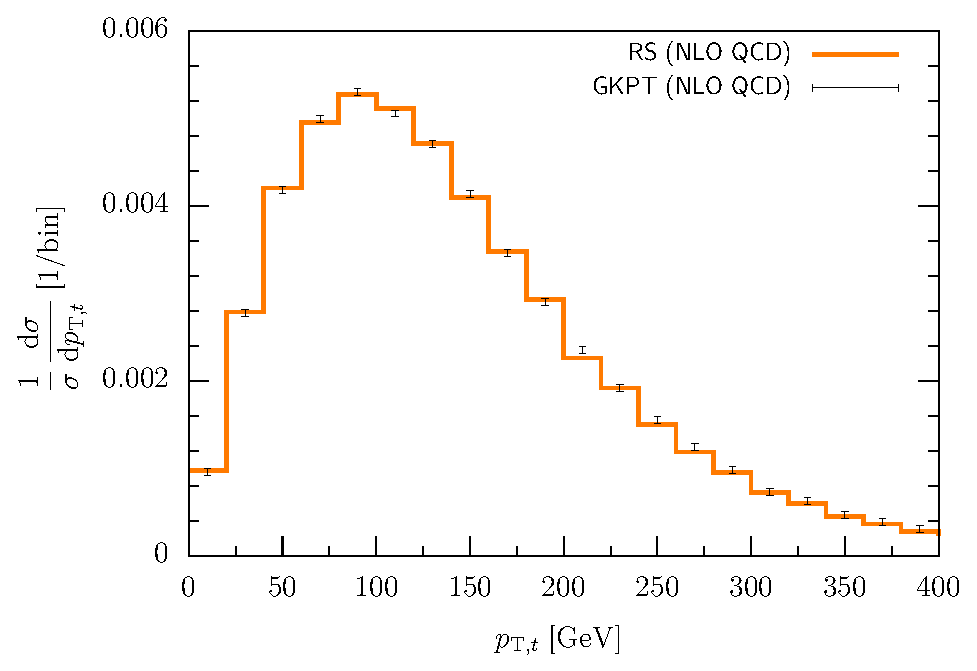
\includegraphics[width=0.49\textwidth]{./Troc_pTtop.eps}
\caption{\label{fig:i} Shape comparison of our results (RS) for stable top quarks and Z boson with the results of Ref.~\cite{Garzelli:2012bn} (GKPT) for 
the transverse momentum spectrum of the top quark at NLO QCD. 
}
\end{figure}

\subsection{Top-Z coupling}   \label{sect:ttzcoupl}
The $\ttbZ$ interaction Lagrangian in the SM can be written as
\begin{equation} \label{L_SM}
\mathcal{L}_{\ttbZ}^{\mrm{SM}} = \mathrm{i} e \, \bar{u}(p_t)\biggl[ \gamma^{\mu} \bigl( \ConeVSM + \gamma_5 \ConeASM \bigr) \biggr]v(p_{\bar{t}}) Z_{\mu}
+ \mathrm{h.c.}
,
\end{equation}
where $e$ is the electromagnetic coupling. The vector and axial couplings are 
\begin{equation}
\begin{split}
\ConeVSM =& \frac{T^3_t - 2Q_t \swsq}{2\sw \cw}, \\
\ConeASM =& \frac{-T^3_t}{2 \sw \cw},  
\end{split}
\end{equation}
where $Q_t = 2/3$ is the top quark charge, $T^3_t=1/2$ and $\theta_w$ is the weak mixing angle. 
% Alternatively, the Lagrangian may be written in terms of left- and right-handed couplings
% \begin{equation} \label{L_SM}
% \mathcal{L}_{\ttbZ}^{\mrm{SM}} = \mathrm{i} e \, \bar{u}(p_t)\biggl[ \gamma^{\mu} \bigl( C_{L}^{\mrm{SM}}\gamma_L + \gamma_R C_{R}^{\mrm{SM}} \bigr) \biggr]v(p_{\bar{t}}) Z_{\mu},
% \end{equation}
% with $\gamma_L=1/2(1-\gamma_{\mu})$, $\gamma_R=1/2(1+\gamma_{\mu})$, and $C_L^{\mrm{SM}}=(T^3 - Q_t \swsq) / (\sw \cw) \\$ and $C_R^{\mrm{SM}}=-Q_t\sw / \cw$. 
New physics contributions to the top-$Z$ couplings are most conveniently introduced by higher dimensional operators 
in the language of effective field theory. 
A minimal set of dimension-6 operators for top quark production and decay have been categorized in Ref.~\cite{AlcarazMaestre:2012vp,AguilarSaavedra:2008zc,Willenbrock?}.
In total there are 91 different operators which can be summarized into 20 different anomalous couplings, if on-shellness and gauge invariance is enforced~\cite{AguilarSaavedra:2008zc}. 
For interactions of a $Z$-boson with top quarks only four anomalous couplings, $C_{1/2,V/A}$, remain and Eq.~\ref{L_SM} becomes
\be
\label{L_NP}
\mathcal{L}_{\ttbZ} = \mathrm{i} e \bar{u}(p_t)\biggl[ \gamma^{\mu} \bigl(C_{1,V} + \gamma_5 C_{1,A} \bigr)
 + \frac{\mathrm{i} \sigma_{\mu \nu} q_{\nu}}{M_Z} 
\bigl(C_{2,V} + \mathrm{i} \gamma_5 C_{2,A} \bigr) \biggr] v(p_{\bar{t}}) Z_{\mu} + \mathrm{h.c.}, 
\ee
with $\sigma_{\mu \nu}=\frac{i}{2} [ \gamma_{\mu},\gamma_{\nu} ]$ and $q_{\nu} = (p_{t}-p_{\bar{t}})_{\nu}$.
The couplings can now be written in terms of the SM contribution plus deviations due to higher dimensional operators
\be
\label{Cone_NP}
   &\ConeV=\ConeV^\mathrm{SM}+\left(\frac{v^2}{\Lambda^2} \right) \mathrm{Re} \left[ C^{(3,33)}_{\phi q} - C^{(1,33)}_{\phi q} - C^{33}_{\phi u}   \right],
   \\
   &\ConeA=\ConeA^\mathrm{SM}+\left(\frac{v^2}{\Lambda^2} \right) \mathrm{Re}\left[  C^{(3,33)}_{\phi q} - C^{(1,33)}_{\phi q} + C^{33}_{\phi u}  \right],
   \nonumber
% \label{Ctwo_NP}
%    &\CtwoV=\CtwoV^\mathrm{SM}+\left(\frac{v^2}{\Lambda^2} \right) \mathrm{Re}\left[ \right],   
%    \quad   \CtwoA=\CtwoA^\mathrm{SM}+\left(\frac{v^2}{\Lambda^2} \right) \mathrm{Re}\left[ \right].   
\ee
where 
\be  
  \label{EFTOp}
  C^{(3,33)}_{\phi q} &=& \mathrm{i} \, (\phi^\dagger \tau^a D_\mu \phi) \, (\bar{t}_\mathrm{L} \gamma^\mu \tau_a t_\mathrm{L})  ,
  \nonumber \\
  C^{(1,33)}_{\phi q} &=& \mathrm{i} \, (\phi^\dagger D_\mu \phi) \, (\bar{t}_\mathrm{L} \gamma^\mu t_\mathrm{L})  ,
  \\
  C^{33}_{\phi u} &=& \mathrm{i} \, (\phi^\dagger D_\mu \phi) \, (\bar{t}_\mathrm{R} \gamma^\mu t_\mathrm{R}). 
  \nonumber
\ee
For the exact definitions of fields in Eq.~\ref{EFTOp} we refer the reader to Ref.~\cite{AguilarSaavedra:2008zc}.
In this paper we will confine ourselfs to the study of the above vector and axial couplings $C_{1,V/A}$, we therefore do not present the expansion of 
the $C_{2,V/A}$ couplings. 
These couplings correspond to the weak magnetic and electric dipole moments of the top quark. 
Their tree level value vanishes in the SM and the first contribution appears at two-loops, with a size of about xxx~\cite{xx}.
Also on the more technical side, the tensor structure that multiplies the $C_{2,V/A}$ couplings introduces the complication of 
non-renormalizable amplitudes at NLO.
While it is straightforward to handle such contributions our current implemenation of the OPP integrand reduction method 
does not allow tensor ranks larger than $N$ for $N$-point loop integrals.
Such an extension of the OPP reduction algorithm has been outlined in the Appendix of Ref.~\cite{}. 
We will come back to this issue in a separate publication and study the phenomenlogical implicications of electroweak dipole moments in $\ttbZ$ production.
\\

We now would like to comment on existing constraints on the $\ttbZ$ couplings.
Clearly, those constraints are not obtained directly through the production of a $Z$-boson in association with top quark pairs.
Instead, they arise from potential deviations which the higher dimensional operators in Eq.~\ref{Cone_NP} introduce to the $\rho$ parameter and the $Z b \bar{b}$ vertex in the SM.
Those parameters are highly constrained through the measurement of the $\varepsilon$ parameters~\cite{},
\be
   \label{epsexp}
   \varepsilon_1^\mathrm{exp} = (5.6 \pm 1.0) \times 10^{-3}, \quad \quad \varepsilon_b^\mathrm{exp} = (-5.8 \pm 1.3) \times 10^{-3}.
\ee
The SM predicts their values as $\varepsilon_1^\mathrm{SM} = (5.21 \pm 0.08) \times 10^{-3} $ and $\varepsilon_b^\mathrm{SM} = -(6.94 \pm 0.15) \times 10^{-3}$~\cite{},
whereas the new physics contributions (\ref{Cone_NP}) introduce the corrections~\cite{}
\be
   \delta \varepsilon_1 &=& \frac{3 m_t^2 G_\mathrm{F}}{2\sqrt{2}\pi^2}  
   \, \mathrm{Re}\left[  C^{(3,33)}_{\phi q}-C^{(1,33)}_{\phi q} + C^{33}_{\phi u} + \mathcal{O}\left(\frac{v^2}{\Lambda^2} \right) \right]
   \left( \frac{v^2}{\Lambda^2} \right) \log\left(\frac{\Lambda^2}{m_t^2}\right),
   \\
   \delta \varepsilon_b &=& -\frac{m_t^2 G_\mathrm{F}}{2\sqrt{2}\pi^2} 
   \, \mathrm{Re}\left[  C^{(3,33)}_{\phi q}-C^{(1,33)}_{\phi q} + \frac14 C^{33}_{\phi u}  \right]
   \left( \frac{v^2}{\Lambda^2} \right)\log\left(\frac{\Lambda^2}{m_t^2}\right).
\ee
The experimental limits in Eq.~\ref{epsexp} can now be used to constrain $C^{(3,33)}_{\phi q}$,  $C^{(1,33)}_{\phi q}$ and $C^{(33}_{\phi u}$.
We will present the numerical results later in Sect.~\ref{} together with our results from $\ttbZ$ production.
We also brielfy note that measurements of the $Z b_\mathrm{L} \bar{b}_\mathrm{L}$ couplings at LEP are in permille level agreement 
with the SM predictions~\cite{}. 
This implies that $  C^{(3,33)}_{\phi q} \approx - C^{(1,33)}_{\phi q}$,
and one of these two operators can be eliminated from Eq.~\ref{Cone_NP}.
% Instead, limits are obtained from the LEP~II measurements of $R_b$ and $A_\mathrm{FB}^{(b)}$ which constrain the $b \bar{b} Z$ couplings.
% $SU(2)_\mathrm{L} \cross U(1)_\mathrm{Y}$ symmetry of the SM can then be used to 

% These contributions introduce deviations to the SM interaction strength such that Eq.~\ref{L_SM} becomes
% \be
% \label{Cone_NP}
%    &\ConeV=\ConeV^\mathrm{SM}+\left(\frac{v^2}{\Lambda^2} \right) \mathrm{Re} \left[ C^{(3,33)}_{\phi q} - C^{(1,33)}_{\phi q} - C^{(33}_{\phi u}   \right],
%    \\
%    &\ConeA=\ConeA^\mathrm{SM}+\left(\frac{v^2}{\Lambda^2} \right) \mathrm{Re}\left[  C^{(3,33)}_{\phi q} - C^{(1,33)}_{\phi q} + C^{(33}_{\phi u}  \right],
%    \\
% \label{Ctwo_NP}
%    &\CtwoV=\CtwoV^\mathrm{SM}+\left(\frac{v^2}{\Lambda^2} \right) \mathrm{Re}\left[ \right],   
%    \quad   \CtwoA=\CtwoA^\mathrm{SM}+\left(\frac{v^2}{\Lambda^2} \right) \mathrm{Re}\left[ \right].   
% \ee
% % the second term is suppressed by a  MARKUS comment: is is not really supressed because q^2/MZ~1, the M is just making it dimensionless
% % mass scale $M$ is typically chosen to be $M_Z$. 
% The $\ConeV$ and $\ConeA$ in Eq.~\ref{C_NP} modify the strength of vector and axial current as predicted by the SM.
% The couplings $\CtwoV$ and $\CtwoA$ induce weak electric and magnetic dipole moments of the top quarks, which vanish at
% tree level in the SM and only receive small corrections starting at two-loops~\cite{}, $C^\mathrm{SM}_{2,V/A} \sim \mathcal{O}(\alpha_s^y\alpha^y)$.
% Higher order corrections enter at ... and lead to a shift of .. \cite{}.
% In an effective field theory for physics beyond the SM, the couplings $\ConeA$ and $\ConeV$ receive contributions from the real part of the difference 
% between two dimension-six operators, 
% as well as the real part of a third operator~\cite{}. 
% The dipole terms $C_{2,V/A}$ are related to a further two dimension-six operators.

% In this paper, we will study sensitivity to the couplings in Eq.~
% interpret the $\ConeV$, $\ConeV$, $\CtwoV$ and $\CtwoA$ as anomalous coupling coefficients which are independent of the kinematics of 
% the top quarks or the $Z$-boson. 
% The dipole terms introduce non-renormalizable amplitudes at NLO, and while it is possible to handle these in the $D$-dimensional unitarity approach \cite{}, 
% it is a non-trivial extension. For this reason, we will focus on the capability of the LHC to constrain the couplings $\ConeA$ and $\ConeV$ in this paper, 
% deferring the analysis of the effects of the dipole couplings $\CtwoV$ and $\CtwoA$ to a future work. We therefore set these couplings to zero throughout 
% the rest of this paper. The anomalous values of the other two couplings are written as relative deviations from their SM values



%Definition of top-Z couplings - vector, axial-vector, left and right handed \\
%Focus of D=4 operators -- D=6 for later (unclear how to implement unitarity for such operators) \\
%Definition of DF1V and DF1A



\section{Results}
\subsection{NLO Results}
%TODO:
%Four distr incl scale bounds (incl at least one of a decay product) at LO, NLO\\
%Comparison with NLO + LO decay \\
%Comparison with 0+1 jet from MadGraph using CKKW merging \\
%Acceptance function = $\sigma_{\mathrm{incl}} / \sigma_{\mathrm{cuts}}$ at LO, NLO\\
%Point out large k-factor with cuts than with fully inclusive \\
In this section we describe the details of our numerical analysis and the results.
We consider the process 
$pp \to \ttb + Z \to t(\to \ell \nu b) \, \bar{t} (\to jj \bar{b}) \, Z(\to \ell \ell)$
and sum over all combinations of leptons $e^\pm, \mu^\pm$.
We choose the following fixed input parameter
\be
 m_t = 173~\GeV,& \quad   m_b = 0~\GeV,&
\nonumber\\
 M_Z =91.1876~\GeV,& \quad  M_W =80.385~\GeV,&
\nonumber\\
 G_\mathrm{F} = 1.166379 \times 10^{-5} \,& \GeV^{-2},  \quad \Gamma_Z = 2.4952~\GeV.&
\ee
Unless otherwise stated, we use MSTW2008 parton distribution functions~\cite{Martin:2009iq} with 
$\alpha_s(M_Z)=0.13939$ and $\alpha_s(M_Z)=0.12018$ at LO and NLO, which we
evolve to the renormalization scale $\mu$ using 1-loop and 2-loop running, respectively.
The LO and NLO scale dependence has already been studied in previous works,
we therefore do not repeat these studies here and adopt the central scale~\cite{Lazopoulos:2008de}  
$\mu_0=m_t + M_Z/2$ 
for $\mu=\mu_\mathrm{ren}=\mu_\mathrm{fact}$.
Since we include NLO QCD corrections to the top quark decay and the hadronically decaying $W$ boson, we need to 
include their total widths up to NLO,
\be
 \Gamma_t^\mathrm{LO} &=& 1.4957~\GeV, \quad \Gamma_t^\mathrm{NLO} = 1.3693~\GeV,
\nonumber\\
 \Gamma_W^\mathrm{LO} &=& 2.0455~\GeV, \quad \Gamma_W^\mathrm{NLO} = 2.1145~\GeV.
\ee
We consider proton-proton collisions at the LHC with a center-of-mass energy of $\sqrt{s}=13~\TeV$.
To account for detector acceptances and trigger we require
\be
\label{selectioncuts}
 \pT^{\ell} \ge 15~\GeV, \quad |y^{\ell}| \le 2.5,
\nonumber\\
 \pT^{j} \ge 20~\GeV, \quad |y^{j}| \le 2.5,
\nonumber\\
 \pT^{\mathrm{miss}} \ge 20~\GeV, \quad R_{\ell j} \ge 0.4.
\ee
Jet are defined by the anti-$k_\mathrm{T}$ algorithm~\cite{Cacciari:2008gp} with $R=0.4$.
With these input parameter and cuts we find the LO and NLO QCD cross sections,
\be
\label{XsecNum}
  \sigma_{\ttb Z}^\mathrm{LO} &= 3.79^{+34\%}_{-25\%}~\mathrm{fb},
  \quad\quad\quad
  \sigma_{\ttb Z}^\mathrm{NLO} &= 5.22^{+15\%}_{-14\%}~\mathrm{fb}
\ee
for the central scale $\mu_0$ which is varied by factors of 2 and $1/2$.
The dependence on the unphysical scale is reduced from approximately $\pm 28\%$ at LO to $\pm 14\%$ at NLO QCD.
Higher order corrections increase the cross section by 38\%, $K= \sigma_{\ttb Z}^\mathrm{NLO} \big/  \sigma_{\ttb Z}^\mathrm{LO}=1.38$.
\begin{figure}[t]
\centering % \begin{center}/\end{center} takes some additional vertical space
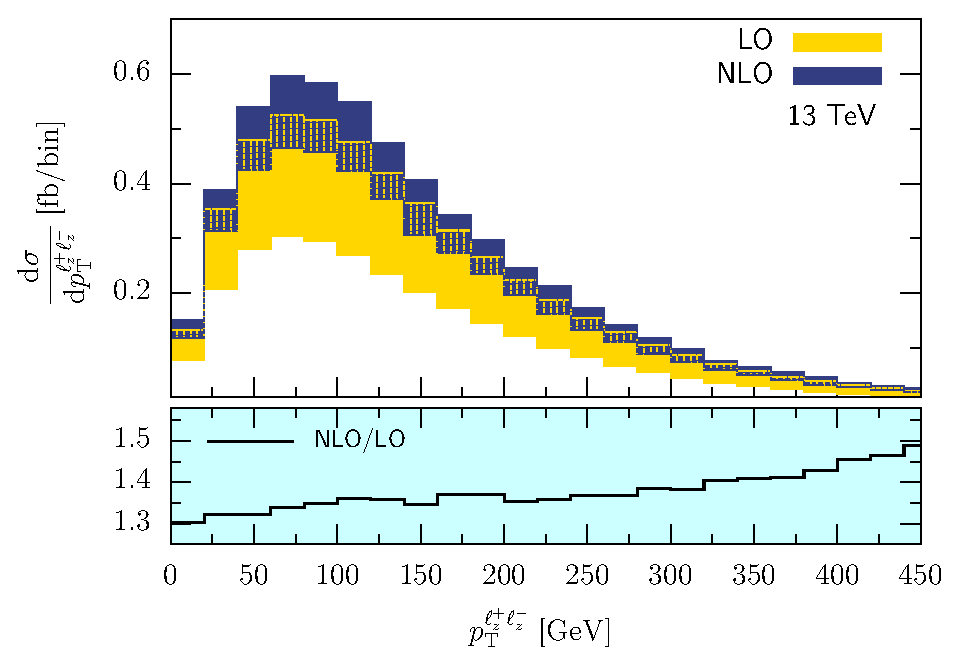
\includegraphics[width=0.49\textwidth]{./LHC_53_Fig12.eps}
% \hfill
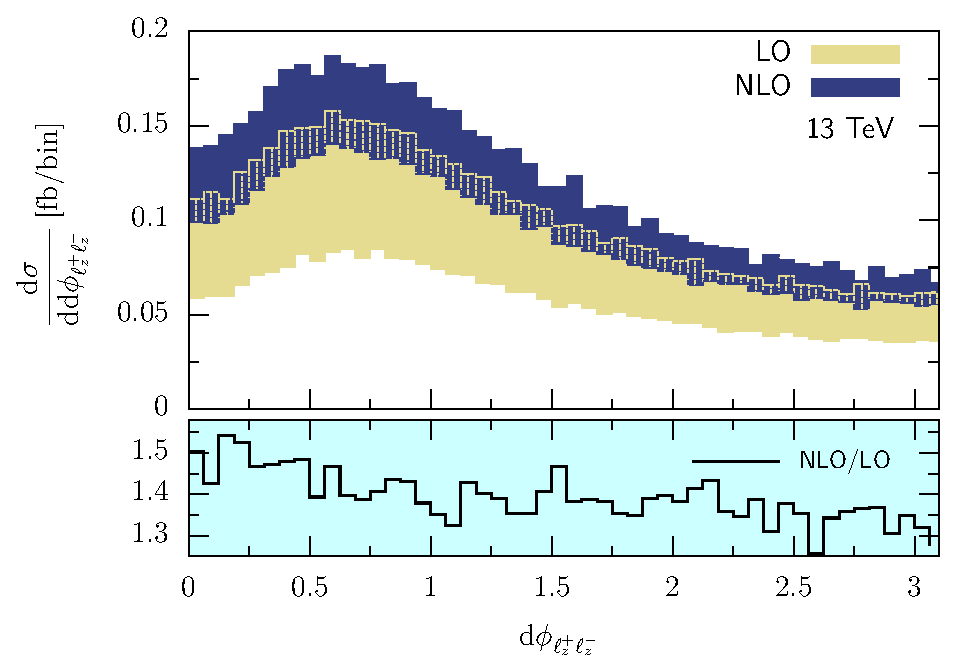
\includegraphics[width=0.49\textwidth]{./LHC_53_Fig17.eps}
\caption{\label{fig:ii} Transverse momentum spectrum (a) and 
in the process $pp \to \ttb + Z \to t(\to \ell \nu b) \, \bar{t} (\to jj \bar{b}) \, Z(\to \ell \ell)$ at the 13~TeV LHC.
The bands represent the LO (light) and NLO (dark) results for scale variation by a factor of two around the central scale $\mu_0$.
}
\end{figure}
We also calculate the acceptance function which is given by the ratio of the cross sections in Eq.~\ref{XsecNum} over the 
cross section without any acceptance cuts, 
\be
  A^\mathrm{LO} = \frac{\sigma_{\mathrm{cuts}}^\mathrm{LO}}{\sigma_{\mathrm{total}}^\mathrm{LO}} = 27.2 \% ,
  \quad\quad\quad
  A^\mathrm{NLO} = \frac{\sigma_{\mathrm{cuts}}^\mathrm{NLO}}{\sigma_{\mathrm{total}}^\mathrm{NLO}} = 30.5 \%.
\ee
We supress dependence on the scale variation because it is almost vanishing in the above ratios.
To estimate uncertainties from parton distribution functions we also evaluate the total cross section
using different sets from CTEQ6L1~\cite{Pumplin:2002vw} and CTEQ10~\cite{Lai:2010vv} at LO and NLO QCD, respectively. 
We find 
\be
\label{XsecNumCTEQ}
  \sigma_{\ttb Z}^\mathrm{LO} &= 3.25^{+34\%}_{-23\%}~\mathrm{fb},
  \quad\quad\quad
  \sigma_{\ttb Z}^\mathrm{NLO} &= 4.86^{+13\%}_{-13\%}~\mathrm{fb}.
\ee
Some short discussion of CTEQ results. Scale var., K, MSTW comparison. Within scale?
We also checked that shape changes can be as large as ... due to the different set of pdf.

\begin{figure}[t]
\centering % \begin{center}/\end{center} takes some additional vertical space
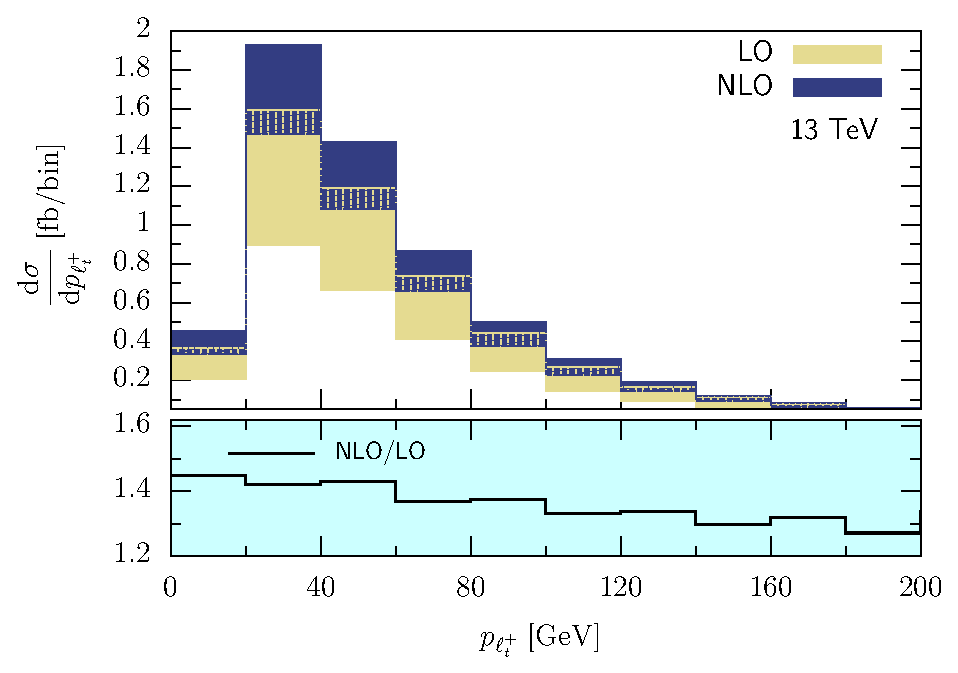
\includegraphics[width=0.49\textwidth]{./LHC_53_Fig01.eps}
\hfill
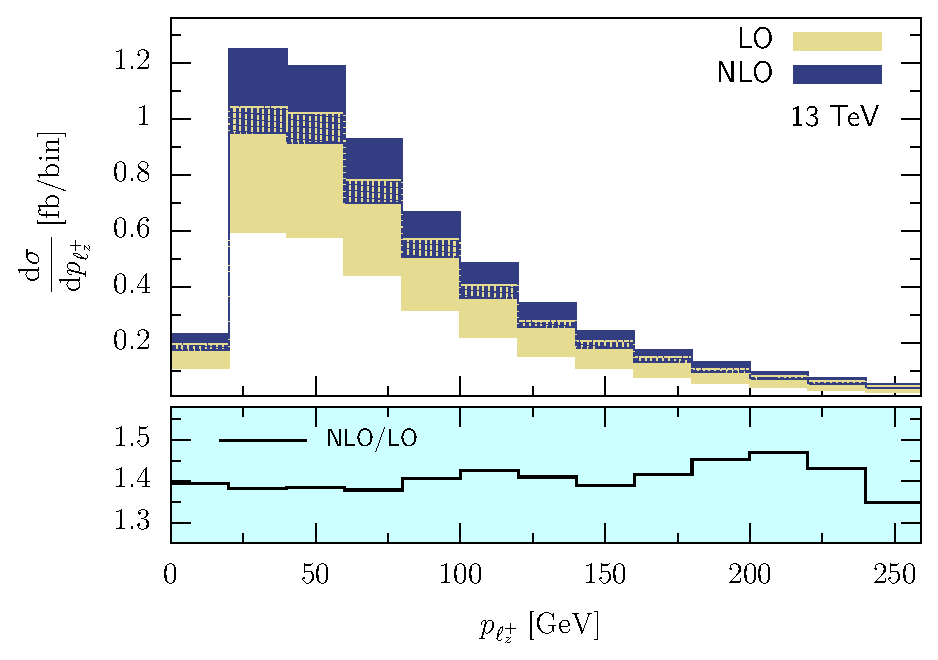
\includegraphics[width=0.49\textwidth]{./LHC_53_Fig03.eps}
\caption{\label{fig:iii} Transverse momentum spectrum of a lepton from the top quark decay~(a) and from the $Z$ boson decay~(b) 
in the process $pp \to \ttb + Z \to t(\to \ell \nu b) \, \bar{t} (\to jj \bar{b}) \, Z(\to \ell \ell)$ at the 13~TeV LHC.
The bands represent the LO (light) and NLO (dark) results for scale variation by a factor of two around the central scale $\mu_0$.}
\end{figure}

Before turning to the $\ttbZ$ coupling analysis, let us discuss some generic kinematic distributions.
Fig.~\ref{fig:ii}a shows the transverse momemtum of two lepton system reconstructing the $Z$ boson.
Similar to the total cross sections we observe a strong reduction in unphysical scale dependence over the entire $\pT$ spectrum.
Scale bands for LO and NLO predictions are comfortably overlapping. 
From this plot we read off an average transverse momemtum of the $Z$ boson of almost 100~GeV with a far extending kinematic tail,
promissing approximately 30 events with $\pT^Z \approx 300~\GeV$ from $300~\mathrm{fb}^{-1}$ at the 13~TeV LHC. 
Fig.~\ref{fig:ii}b shows the azimuthal opening angle between the two leptons from the $Z$ boson decay.
This observable has been proven to be a good analyzer of the $\ttbZ$ couplings~\cite{Baur:2004uw} and we wil consider it in the following analysis.
The differential $K$-factor in the lower pane of this plot shows shape changes in the range of 10~\% due to higher order corrections.
Shape changes that arise from higher order corrections in the decay matrix elements are shown in the dashed line and amount up to xx\%.



In Fig.~\ref{fig:iii}a and Fig.~\ref{fig:iii}b we compare the transverse momentum between the leptons from the top quark and $Z$ boson decay.
We find that leptons from the $Z$ boson have a typically harder spectrum. 
This is already true for LO while significatly different $K$-factors enhance this behavior even further at NLO.

%tagCMSdata
% \subsection{Top-Z coupling results from current CMS data}
\subsection{Coupling extrapolation and first results from current CMS data}
\label{sect:CMS}

In this section and the next, we will use our calculation to investigate the constraints that can be placed on top-Z couplings, using both existing and anticipated LHC data. 
To do so, we need to determine how normalization and shapes depend on variations of the couplings. 
Hence total cross-sections and differential distributions need to be calculated for a large grid of $C_{1,V}$ and $C_{1,A}$ values. 
This is simple enough at LO, and while it is still feasible at NLO, it does place a strain on computing resources. 
As a convenient alternative, we note that $\ttbZ$ production and decay amplitude at LO or NLO QCD can be written as
\begin{equation}
  \mathcal{M} = \mathcal{M}_0 +  \ConeV \mathcal{M}_\mathrm{V} +  \ConeA \mathcal{M}_\mathrm{A},
\end{equation}
with the coefficients $\mathcal{M}_i$ encoding both the kinematics and all couplings other than the top-Z coupling. 
The differential cross-section is then dependent on six coupling stuctures, and can be written as
\begin{equation}
\label{couplfit}
  d\sigma = s_0 +s_1C_{1,V} + s_2C_{1,V}^2 +s_3 C_{1,A}+s_4C_{1,A}^2+s_5C_{1,V}C_{1,A}.
\end{equation}
Evaluating the cross-section for six values of $(C_{1,V},C_{1,A})$ allows us to solve for the coefficients $s_i$. 
These can then be used to extrapolate results for any values of $C_{1,V}$ and $C_{1,A}$. 
Furthermore, this fitting procedure can not only be done for the total cross-section but also bin-by-bin for a given distribution, 
retaining the effects of spin correlations and selction cuts.
As a check of this approach, we have evaluated the cross-sections and distributions for a few points in the $(C_{1,V},C_{1,A})$ parameter space, 
both by an explicit calculation and by using the fit for the $s_i$ coefficients. Excellent agreement is found in all cases. 
As an example, we show one comparison in Fig.~\ref{fig:iv} for the  $\Delta \phi_{\ell^+_z \ell^-_z}$ distribution, which we will later use in the coupling analysis.
The relative shifts in the couplings are given by
\be
%\begin{split}
\DConeV =  \frac{\ConeV}{\ConeVSM}-1 ; \hspace{2cm} \DConeA = \frac{\ConeA}{\ConeASM}-1.
\ee
As can be seen in Fig.~\ref{fig:iv}, the overall normalization and the shape are correctly reproduced by the fitting procedure.
\begin{figure}[t]
\centering % \begin{center}/\end{center} takes some additional vertical space
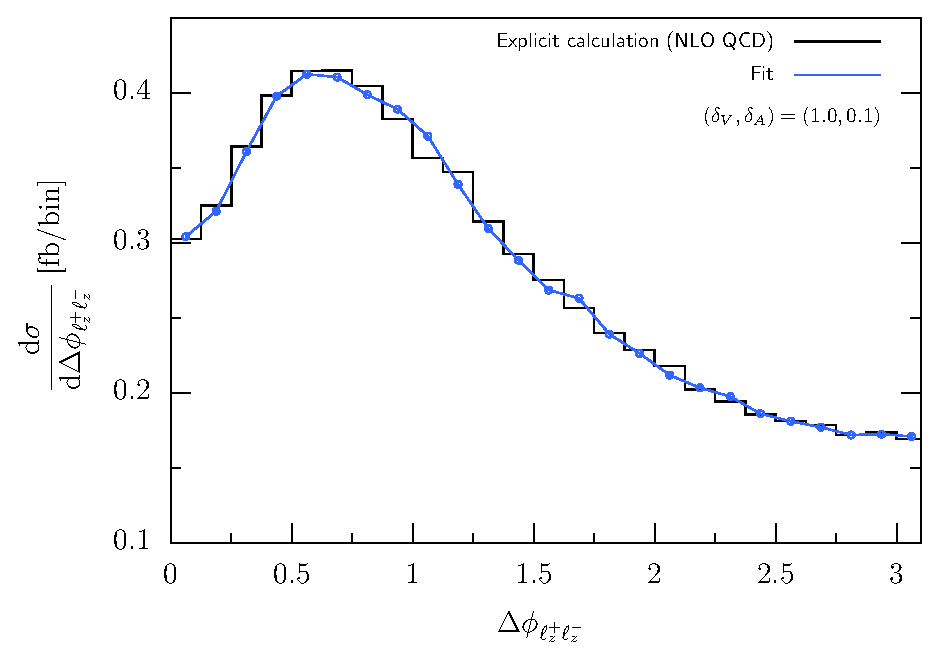
\includegraphics[width=0.49\textwidth]{./LHC_53_Fig17d.eps}
\caption{\label{fig:iv} Validation of our fitting procedure. Shown is the $\Delta \phi_{\ell^+_z \ell^-_z}$ distribution from an explicit NLO QCD calculation 
for the non-SM coupling choice $(\DConeV,\DConeA)=(1.0,0.1)$, and from the fit described in Eq.~3.8. }
\end{figure}

{\bf MARKUS NOTE: I think we have to be careful with the word observed. This is typically only used for 5sigma signals, which is not the case here at all.}
We turn now to an analysis based on current LHC data. The production of $\ttbZ$ has been observed at the $\sqrt{s}=7$ TeV run at the LHC, 
with CMS observing nine events~\cite{Chatrchyan:2013qca}, and ATLAS observing one event with more stringent selection criteria~\cite{ATLAS-CONF-2012-126}. 
This enables ATLAS to place an upper bound on the $\ttbZ$ cross-section, 
while CMS is able to determine $\sigma_{\ttbZ} = 0.28^{+0.14}_{-0.11}~\mathrm{(stat.)}^{+0.06}_{-0.03}~ \mathrm{(sys.)}$~pb. 
Clearly, error bars from these very first measurements are huge nevertheless they are consistent with the NLO QCD prediction of 0.137~pb in Ref.~\cite{Garzelli:2011is} or this work. 
In spite of the low number of events and correspondingly high statistical error, it is instructive to use this overall cross-section to place bounds on the top-Z couplings. 
This constitutes the first direct constraints on these couplings.
We perform a simple $\chi^2$-test 
\begin{equation}
\chi^2 = \frac{f \sigma_{\mathrm{pred}} - \sigma_{\mathrm{CMS}}}{\Delta \sigma_{\mathrm{CMS}}},
\end{equation}
where $\sigma_{\mathrm{pred}}=\sigma_{\mathrm{pred}}(C_{1,V},C_{1,A})$ is the predicted cross-section at LO or NLO, 
$\sigma_{\mathrm{CMS}}$ is the cross-section measured by CMS, with error $\Delta \sigma_{\mathrm{CMS}}$ taken by adding the larger 
statistical and systematic errors in quadrature, $\Delta \sigma_{\mathrm{CMS}}=\sqrt{0.14^2+0.06^2}$. 
The factor $f$ takes into account the uncertainties in the theoretical predicion due to the scale and pdf choices. 
It is defined as~\cite{Baur:2004uw,Baur:2005wi}
 \begin{equation}
f = \left\{ 
\begin{array} {l l}
(1+\Delta N)  & \quad \mathrm{if}~ f^* > 1 + \Delta N \\
1/(1+\Delta N)  & \quad \mathrm{if}~ f^* < 1/(1 + \Delta N) \\
f^* & \quad \mathrm{if}~ 1/(1 + \Delta N) < f^* < 1+\Delta N,
\end{array} \right.\ 
\end{equation}  
where the $f^*$ minimizes $\chi^2$, $f^* = \sigma_{\mathrm{CMS}} / \sigma_{\mathrm{pred}}$, and $\Delta N$ is the theoretical  uncertainty. 
This strategy is similar to treating $f$ as a nuisance parameter and marginalizing over it; however, we do not allow it complete freedom, 
but instead require it to be within the bounds of the theoretical uncertainty. 
In determining $\Delta N$, we found in the previous section scale uncertainties of 30\% at LO and 15\% at NLO QCD.
Uncertainties related to using different parton distribution functions amount to 17\% at LO and 7\% at NLO. 
Since the latter uncertainties are comfortably within the variation of renormalization and factorization scales, we 
choose here and in the following analysis $\Delta N = 0.30$ at LO and $\Delta N = 0.15$ at NLO.
% we use a pdf uncertainty of 5\% and a scale uncertainty of 30\% at LO and 15\% at NLO, as found in the previous section. 
% We sum these uncertainties linearly to obtain $\Delta N = 0.35$ at LO and $\Delta N = 0.20$ at NLO. 

Figure~\ref{fig:v} shows the results of the $\chi^2$-test obtained from our leading order (left) and next-to-leading order (right) calculations
which relate the total cross section with the $\ttbZ$-couplings.
In the plane of relative deviations of vector and axial couplings, the point $(\DConeV,\DConeA)=(0.0,0.0)$ corresponds to the SM value.
The broad black band represents coupling choices which are indistinguishable from the SM prediction within our simple analysis.
With the given experimental data set those couplings can extend to $(\DConeV,\DConeA)=(-600\%,-200\%)$.
By comparing left and right plots we clearly notice the stronger constraints when NLO input is used.
In particular, the region around the point $(\DConeV,\DConeA)=(-1.0,-1.2)$ can be much stronger excluded at NLO. 
Since this area corresponds to very small cross sections, next-to-leading order data favors the experimental observation of the $\ttbZ$ final state even more.
Of course, the obtained limits have to be interpreted with care since very few events have been observed by the experiments so far.
Only a larger data set and detailed analysis of backgrounds and detector effects will provide more reliable constraints on the $\ttbZ$-couplings.
We still belive that these results are interesting to consider, especially when being put in context with limits
obtained from the future high-energy LHC which we study in the next section.



\begin{figure}[t]
\centering % \begin{center}/\end{center} takes some additional vertical space
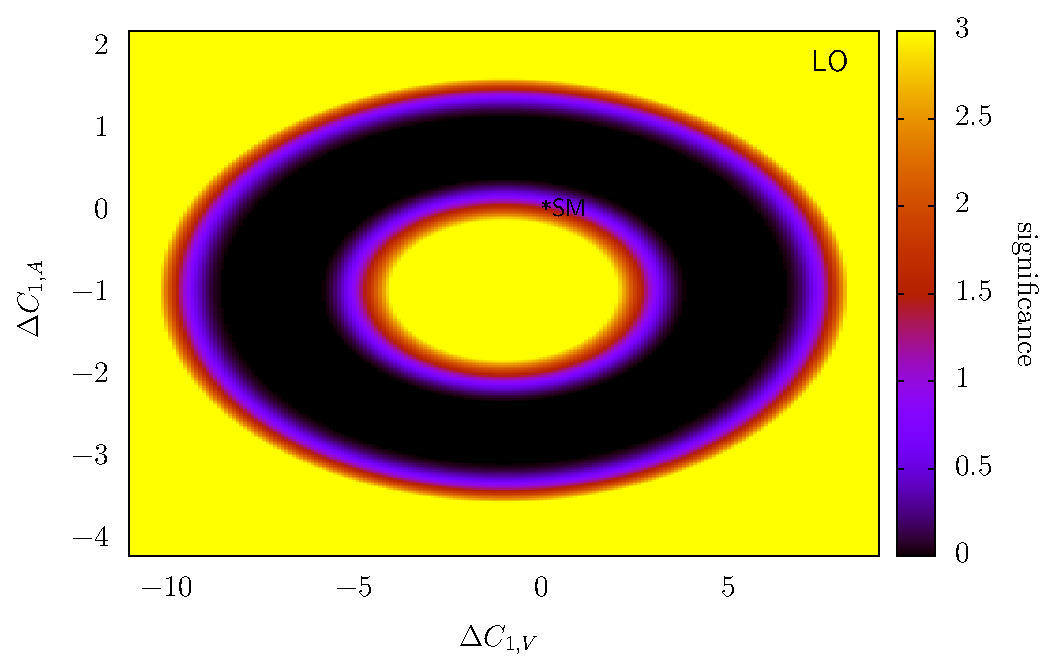
\includegraphics[width=0.495\textwidth]{./CMSLO_Delta0.40_0213.eps}
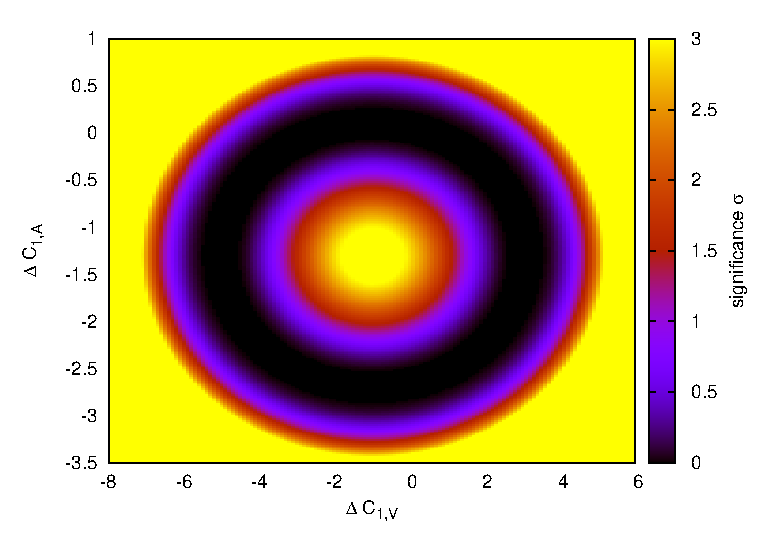
\includegraphics[width=0.495\textwidth]{./CMSNLO_Delta0.20_0213.eps}
\caption{\label{fig:v}
Significance as a function of relative deviations for vector and axial couplings wrt. the SM value. 
The limits are obtained from the first measurement of the $\ttbZ$ cross section by CMS~\cite{Chatrchyan:2013qca}. 
The left~(right) plot shows the limits obtained from LO~(NLO QCD) input.
}
\end{figure}

\subsection{Top-Z coupling constraints from future LHC runs}




We now move on to study future constraints that analyses of the high energy LHC run can place on the top-Z coupling.
For this, we assume a centre-of-mass energy of $\sqrt{s}=13$~TeV and consider projections for an integrated luminosity of
$30\, \invfb$, $300\, \invfb$, and $3000\, \invfb$. 
We focus on the trileptonic final state and employ the azimuthal angle between the leptons originating
from the $Z$ decay to perform our analysis.
This angle has been identified as being particularly sensitive to the top-Z coupling in Ref.~\cite{Baur:2004uw}.
We already discussed the strong reduction in scale uncertainty when going from LO to NLO QCD for this observable.
Here, in Fig.~\ref{fig:vi}(a) we show the effect of NLO QCD corrections on the shape of the normalized $\Delta \phi_{\ell\ell}$ distribution.
Higher order effects tend to shift events from larger to smaller opening angles.
In Fig.~\ref{fig:vi}(b) we show that similar shape changes can arise due to variations of the vector and axial $\ttbZ$-couplings.
This emphasizes the importance of precise predictions since missing higher order effects might be misinterpreted as deviations from the SM.
To illustrate that the $\Delta \phi_{\ell\ell}$ shape is a useful discriminator for our coupling analysis, we have chosen 
values $\delta_V$ and $\delta_A$ in Fig.~\ref{fig:vi}(b) such that the total cross sections approximately coincide with the SM value.
Hence, a measurement of the rate alone would not reveal the deviations from their Standard Model value.
% , and a combination of normalization and shape information provides the best sensitivity.
 


\begin{figure}[t]
\centering % \begin{center}/\end{center} takes some additional vertical space
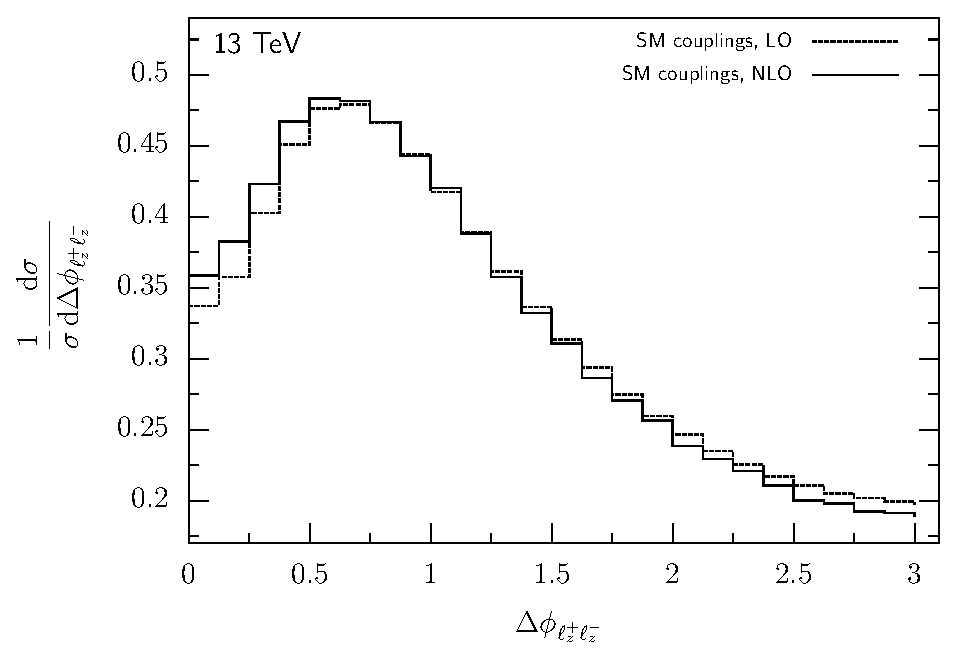
\includegraphics[width=0.45\textwidth]{./LHC_53_Fig17a.eps}
\hfill
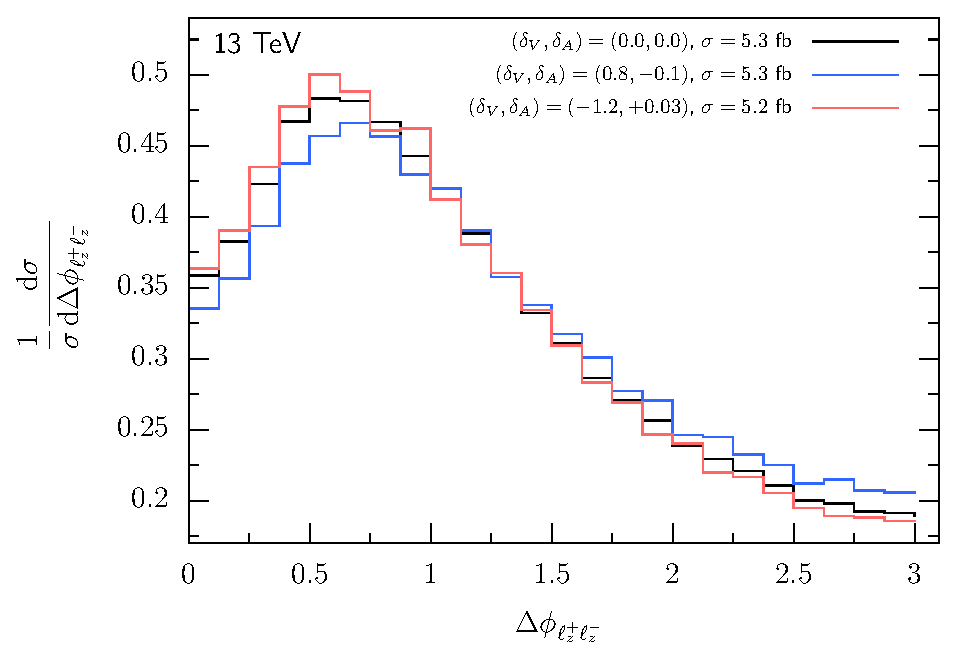
\includegraphics[width=0.45\textwidth]{./LHC_53_Fig17b.eps}
\caption{\label{fig:vi}
Normalized distributions of the azimuthal opening angle of the opposite sign leptons from the $Z$ boson decay at the 13~TeV LHC.
In the left Figure~(a), shapes of LO and NLO QCD predictions are compared for SM $\ttbZ$-couplings.
Shape changes due to deviations from the SM values are shown in the right Figure~(b).
}
\end{figure}



Let us now outline the basic idea of our statistical analysis.
We are interested in answering the question: What are the bounds that can be placed on top-Z couplings? 
Obviously, the answer will depend on the assumed integrated luminosity of the data sample as well as theoretical and experimental uncertainties. 
However, we emphasize again that we do not take experimental effects into account apart from the cuts in Eq.~\ref{selectioncuts} to account for detector acceptances.
Since at the current point in time there is no experimental data available, we assume the SM prediction as our null hypothesis 
$\mathcal{H}_{\mathrm{SM}}$ ($\DConeV,\DConeA)=(0,0)$,
against which we test alternative hypotheses $\Halt$ with $(\DConeV,\DConeA) \ne (0,0)$.
Once experiments have accumulated real events, the alternative hypothesis can be replaced by observed data to test for consistency with the SM prediction. 
The null hypothesis could then be replaced by  other points in $(\DConeV,\DConeA)$ parameter space, and tested against the data. 
This will enable the exclusion of parts of the parameter space at a given confidence level (e.g. 3-$\sigma$). 
Assuming that the data agree with the SM, 
% and ignoring experimental effects which may be significant, 
the bounds on the top-Z coupling 
obtained in this section should approximate those obtained from real data in the future. 
We begin by constructing two likelihood functions $\mathcal{L}_{\SM}$ and $\mathcal{L}_{\alt}$ which allow us to define a test 
statistic $\Lambda = \log \left( \mathcal{L}_{\SM} / \mathcal{L}_{\alt} \right)$.
% Assuming a fixed integrated luminosity, we now generate a number of events for the two hypotheses $\mathcal{H}_{\mathrm{SM}}$ and $\Halt$ based on our NLO QCD predictions for $\Delta \phi_{\ell\ell}$.
% Based on our NLO QCD predictions for $\Delta \phi_{\ell\ell}$, we now generate two event samples for a fixed integrated luminosity assuming that either $\mathcal{H}_{\mathrm{SM}}$ or $\Halt$ is true.
We now generate two event samples for a fixed integrated luminosity assuming that either $\mathcal{H}_{\mathrm{SM}}$ or $\Halt$ is true.
The test statistic $\Lambda$ can be evaluated for these two event samples, and 
repeating this evaluation in a large number of pseudo experiments provides the probability distributions $P(\Lambda|\mathcal{H}_{\mathrm{SM}})$ or $P(\Lambda|\Halt)$.
The overlap of these two probability distributions can be used to define the type-I error for rejecting $\mathcal{H}_{\mathrm{SM}}$ in favor of $\Halt$, even though $\mathcal{H}_{\mathrm{SM}}$ is true.
This error can finally be translated into the more familiar confidence level in terms of standard deviations.



In the following we will describe the procedure outlined above more precisely and illustrate how NLO QCD input can be used.
The starting point is the binned likelihood function 
\be
\label{lili}
   \mathcal{L}(\mathcal{H}|\vec{n}) = \prod_{i=1}^{N_\mathrm{bins}} P_i(n_i|\nu_{i}^\mathcal{H})
\ee
with the Poisson distribution $P_i$ for $n_i$ events in the $i$-th bin, given the expected value $\nu_{i}^\mathcal{H}$ for hypothesis $\mathcal{H}$. 
% This expected value is obtained by multiplying the differential cross-section in bin $i$ by the assumed luminosity.
%The starting point is the binned likelihood function 
%\be
%\label{lili}
%   \mathcal{L}(\mathcal{H}_a,\vec{n}|\mathcal{H}_t,\vec{\nu}) = \prod_{i=1}^{N_\mathrm{bins}} P_i(n_i^{\mathcal{H}_a}|\nu_{i}^{\mathcal{H}_t})
%\ee
%with the Poisson distribution $P_i$ for $n_i$ events in the $i$-th bin, given the expected value $\nu_{i}^{\mathcal{H}_a}$ for the assumed hypothesis $\mathcal{H}_a$. 
%The values $\nu_i^{\mathcal{H}_t}$ are drawn from the test hypothesis $\mathcal{H}_t$. The values $\nu_i$ are obtained by multiplying the differential cross-section in bin $i$ by the assumed luminosity.
Consequently the two log-likelihood functions for the SM and the alternative hypthesis read
\be
\label{lilifunct}
\begin{split}
  \log\mathcal{L}(\HSM |\vec{n}_\mathrm{obs})  =& \sum_{i=1}^{N_\mathrm{bins}} \bigl[ n_{i,\mathrm{obs}}\log(\nu_i^{\SM}) -\log(n_{i,\mathrm{obs}}!) -\nu_i^{\SM}  \bigr], \\
  \log\mathcal{L}(\Halt|\vec{n}_\mathrm{obs})  =& \sum_{i=1}^{N_\mathrm{bins}} \bigl[ n_{i,\mathrm{obs}}\log(\nu_i^{\alt})-\log(n_{i,\mathrm{obs}}!) -\nu_i^{\alt} \bigr],
\end{split}
\ee
%Consequently there are the log-likelihood functions for a test hypothesis $\mathcal{H}_t$ under the assumption of a hypothesis $\mathcal{H}_a$
%\be
%\label{lilifunct}
%\begin{split}
%  \log\mathcal{L}(\mathcal{H}_a,\vec{n}|\mathcal{H}_t,\vec{\nu})  = \sum_{i=1}^{N_\mathrm{bins}} \bigl[ n_i^{\mathcal{H}_a}\log(\nu_i^{\mathcal{H}_t}) -\log(n_i^{\mathcal{H}_a}!) -\nu_i^{\mathcal{H}_t}  \bigr],% \\
%  \log\mathcal{L}(\HSM,\vec{n}|\HSM)  =& \sum_{i=1}^{N_\mathrm{bins}} \bigl[ n_i^{\SM}\log(\nu_i^{\SM}) -\log(n_i^{\SM}!) -\nu_i^{\SM}  \bigr], \\
%  \log\mathcal{L}(\HSM,\vec{n}|\Halt)  =& \sum_{i=1}^{N_\mathrm{bins}} \bigl[ n_i^{\SM}\log(\nu_i^{\alt}) -\log(n_i^{\SM}!) -\nu_i^{\alt}  \bigr], \\
%  \log\mathcal{L}(\Halt,\vec{n}|\HSM)  =& \sum_{i=1}^{N_\mathrm{bins}} \bigl[ n_i^{\alt}\log(\nu_i^{\SM}) -\log(n_i^{\alt}!) -\nu_i^{\SM}  \bigr], \\
%  \log\mathcal{L}(\Halt,\vec{n}|\Halt)  =& \sum_{i=1}^{N_\mathrm{bins}} \bigl[ n_i^{\alt}\log(\nu_i^{\alt}) -\log(n_i^{\alt}!) -\nu_i^{\alt}  \bigr], 
%  \log\mathcal{L}(\Halt|\vec{n}_\mathrm{obs})  =& \sum_{i=1}^{N_\mathrm{bins}} \bigl[ n_{i,\mathrm{obs}}\log(\nu_i^{\alt})-\log(n_{i,\mathrm{obs}}!) -\nu_i^{\alt} \bigr],
%\end{split}
%\ee
%where $n_{i,\mathrm{obs}}$ is the observed number of events in the $i$-th bin of the $\Delta \phi_{\ell\ell}$ distribution. 
Eqs.~\ref{lilifunct} allow us to construct the test statistic as the log-likelihood ratio
\be
\begin{split}
  \Lambda(\vec{n}_\mathrm{obs}) =& \log \biggl( \mathcal{L}(\HSM |\vec{n}_\mathrm{obs})  \big/ \mathcal{L}(\Halt|\vec{n}_\mathrm{obs})  \biggr)  \\
                                =& \sum_{i=1}^{N_\mathrm{bins}} \biggl[ n_{i,\mathrm{obs}}\log \biggl( \frac{\nu_i^{\SM}}{\nu_i^{\alt}} \biggr) -\nu_i^{\SM} + \nu_i^{\alt} \biggr],
\end{split}
\ee
where $\vec{n}_{\mrm{obs}}$ are generated by a Poisson distribution of $\nu_i^{\SM}$ and $\nu_i^{\alt}$
from the $\Delta \phi_{\ell\ell}$ histograms for $\HSM$ and $\Halt$, respectively.
% , yielding $\vec{n}_{\SM}$ and $\vec{n}_{\alt}$.
\begin{figure}[t]
\centering % \begin{center}/\end{center} takes some additional vertical space
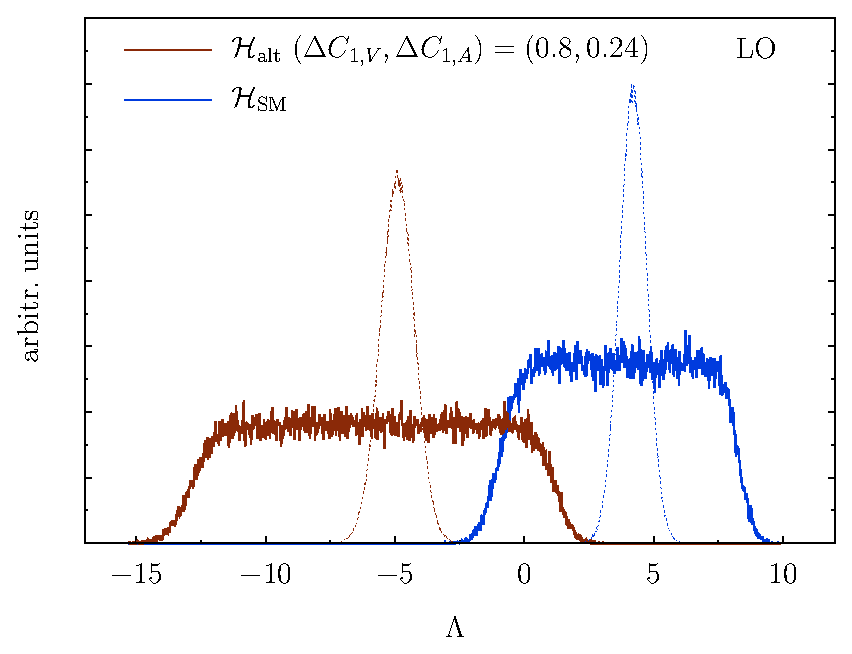
\includegraphics[width=0.49\textwidth]{./LogLikelihoods_LO.eps}
\hfill
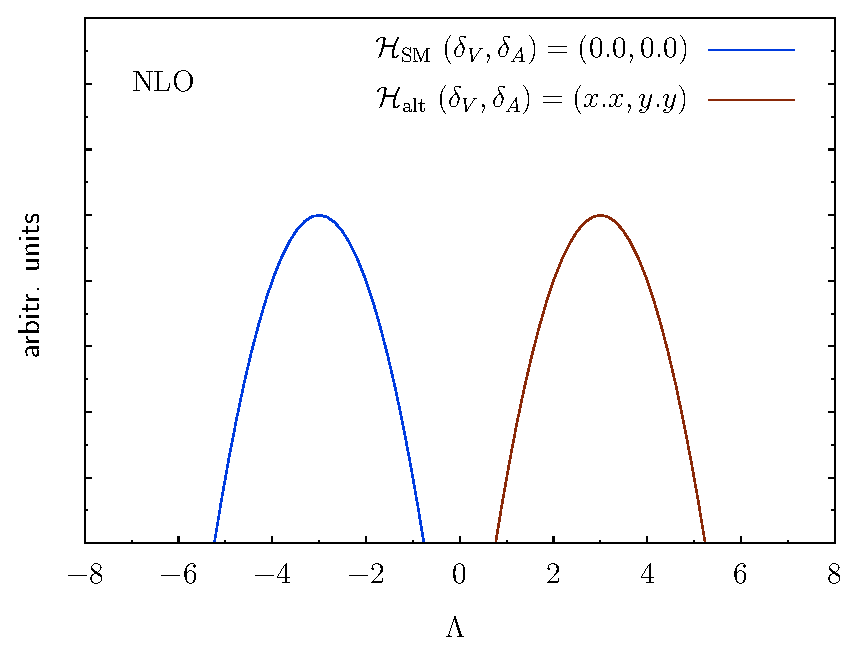
\includegraphics[width=0.49\textwidth]{./LogLikelihoods_NLO.eps}
\caption{\label{fig:vii}
Probability distributions of the log-likelihood ratio $\Lambda$ assuming that the observed events follow the SM hypothesis (red) or an alternative hypothesis (blue) 
with $(\DConeV,\DConeA)=(0.8,0.24)$.
The solid lines include statistic and systematic uncertainties as described in the text, whereas the dashed lines only include statistic uncertainties.
The left plot shows the separating power using LO input with $\Delta_\mathrm{syst.}=30\%$, 
the right plot is obtained at NLO QCD with $\Delta_\mathrm{syst.}=15\%$, assuming $\sqrt{s}=13\,\TeV$ and $\mathcal{L}=300\,\invfb$.
}
\end{figure}
%\be
%\begin{split}
%  \Lambda(\HSM) =&  \, \log \biggl( \mathcal{L}(\HSM,\vec{n}|\HSM,\vec{\nu})  \big/ \mathcal{L}(\HSM,\vec{n}|\Halt,\vec{\nu})  \biggr)  \\
%                                =& \, \sum_{i=1}^{N_\mathrm{bins}} \biggl[ n_{i}^{\SM}\log \biggl( \frac{\nu_i^{\SM}}{\nu_i^{\alt}} \biggr) -\nu_i^{\SM} + \nu_i^{\alt} \biggr],
%\end{split}
%\ee
%and similarly
%\be
%\begin{split}
%  \Lambda(\Halt) =& -2 \, \log \biggl( \mathcal{L}(\Halt,\vec{n}|\HSM,\vec{\nu})%  \big/ \mathcal{L}(\Halt,\vec{n}|\Halt,\vec{\nu})  \biggr)  \\
%                                =& -2\, \sum_{i=1}^{N_\mathrm{bins}} \biggl[ n_{i}^{\alt}\log \biggl( \frac{\nu_i^{\SM}}{\nu_i^{\alt}} \biggr) -\nu_i^{\SM} + \nu_i^{\alt} \biggr],
%\end{split}
%\ee
%This function $\Lambda$ can now be evaluated with $\vec{n}$ events which are distributed according to the 
% $\Delta \phi_{\ell\ell}$ distribution of either the SM hypothesis or the alternative hypothesis. 
Repeating this procedure for a large number of pseudo-experiments yields the two probability distributions of $\Lambda(\vec{n}_\mathrm{SM})$ and $\Lambda(\vec{n}_\mathrm{alt})$. 
%Repeating this procedure for a large number of pseudo-experiments yields the two probability distributions  $P(\Lambda|\HSM)$ and $P(\Lambda|\Halt)$.
An example of two such probability distributions is shown in Figs.~\ref{fig:vii} for LO and NLO QCD, respectively. 
For a given value $\hat{\Lambda}$, the probability of accepting $\mathcal{H}_{\alt}$ even though $\mathcal{H}_{\SM}$ is correct (type-I error) is
\begin{equation}
    \alpha = \int^{\hLambda}_{-\infty} \mathrm{d}\Lambda \; P(\Lambda | {\HSM}).
\end{equation}
Similarly, the probability of accepting $\mathcal{H}_{\SM}$ even though $\mathcal{H}_{\alt}$ is correct (type-II error) is given as 
\begin{equation}
    \beta = \int_{\hLambda}^{\infty} \mathrm{d}\Lambda \; P(\Lambda|\Halt).
\end{equation}
We define $\hLambda$ such that $\alpha=\beta$, i.e. there is equal chance of {\it incorrectly} rejecting one hypothesis in favor of the other. 
The value $\alpha(\hLambda)$ is then a measure of statistical discrimination between the two hypotheses. 
It can be translated into the more familiar number of standard deviations by 
\begin{equation}
\sigma = \sqrt{2} \, \erf^{-1}(1-\alpha),
\end{equation}
where $\erf^{-1}$ is the inverse error function. 

The above discussion made so far no mention of systematic uncertainties.
In this work we would like to include the leading theoretical uncertainties from unphysical scale dependence and errors associated with parton distribution functions.
For simplicity we neglect experimental systematics such as efficiencies or momentum smearing effects.
Note however that we include realistic detector acceptances through the cuts in Eq.~\ref{selectioncuts}.
Statistical fluctuations are obviously included through the Poisson distribution in Eq.~(\ref{lili}).
Following Ref.~\cite{Conway}, we include the theoretical uncertainties 
by integrating the expected number of events over the range $(1 \pm \Delta_\mathrm{unc.})$ 
when generating the pseudo-experiments.
This is achieved by modifying the likelihood function in Eq.~\ref{lili} according to
\be
  \mathcal{L}(\mathcal{H}|\vec{n}) \to \mathcal{L}(\mathcal{H}|\vec{n})  \,\times\, \mathcal{G} \left( \nu_i^\mathcal{H} | \tilde{\nu}_i^\mathcal{H}  (1 \pm \Delta_\mathrm{unc.}) \right),
\ee
where we choose $\mathcal{G}$ to be a normalized function uniformly distributed around $\tilde{\nu}_i^\mathcal{H}$ with spead $\Delta_\mathrm{unc.}$.
The value of $\tilde{\nu}_i^\mathcal{H}$ is determined by the cross section and the assumed luminosity.
As mentioned in the previous Section, we choose $\Delta_\mathrm{unc.} = 30\%$ at LO
and $\Delta_\mathrm{unc.} = 15\%$ at NLO QCD in our analysis.
The effect of these additional uncertainties is to broaden the distributions in $\Lambda$, 
resulting in a larger overlap between the two distributions, and consequently a larger $\alpha$ value and less discriminatory power between the two hypotheses. 
This feature is clearly visible in Fig.~\ref{fig:vii}, when comparing the solid with the doted curves. 
Contrasting the LO results in Fig.~\ref{fig:vii}(left) with the NLO result (right) shows that 
the lower uncertainty associated with the NLO prediction allows for significantly better statistical discrimination between the hypotheses.
Also the increase of the NLO cross section due to the $K$-factor of $\approx1.4$ leads to a larger number of expected events and therefore to smaller statistical uncertainties.


\begin{figure}[t]
\centering
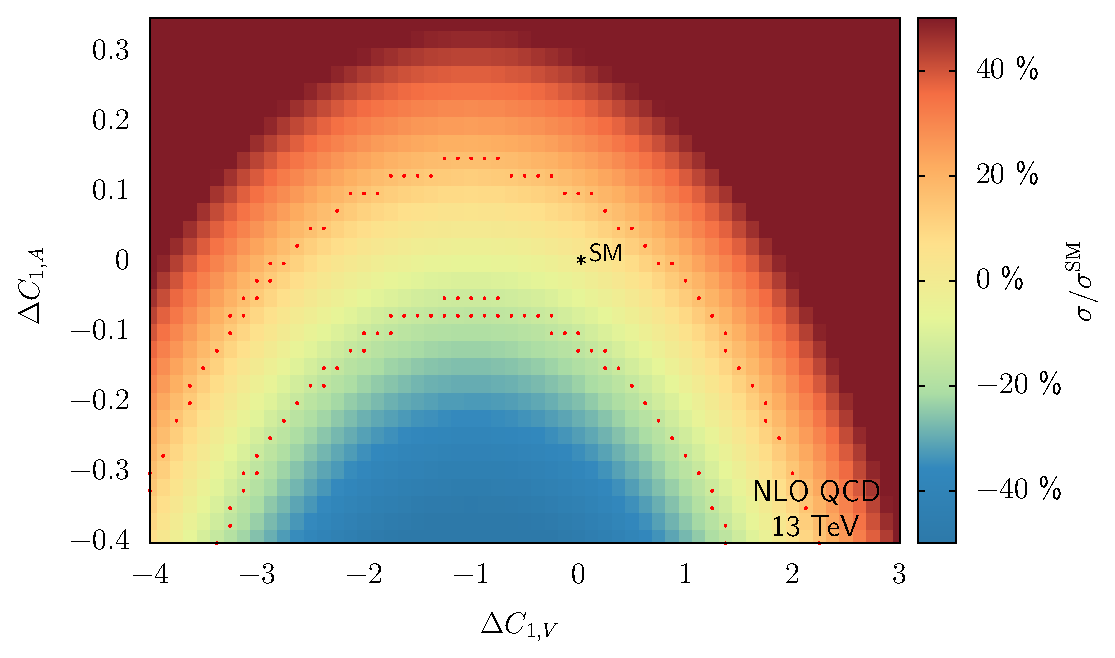
\includegraphics[scale=0.6]{LHC_53_SigmaNLO.eps}
\caption{ \label{fig:viii} Relative deviations of the NLO QCD cross section as a function of relative shifts in vector and axial couplings wrt. the SM.
The grid of $ 80 \times 40 $ coupling choices is obtained from the fit described in Eq.~3.8. }
\end{figure}

We now present the results of our analysis in Figs.~\ref{fig:viii} and~\ref{fig:ix}.
The first Figure shows the NLO QCD cross section relative to the SM cross section 
including selection cuts of Eq.~\ref{selectioncuts} for a wide range of top-Z vector and axial couplings.
This grid of 3200 NLO QCD cross sections is generated with the fit described around Eq.~\ref{couplfit}, at low computational cost.
We find that within the given range the cross section varies by about $\pm 50\%$.
Note that the remaining scale unceratinty at NLO QCD was found to be $\sim 15\%$ which roughly corresponds to the area inside the dotted band in Fig.~\ref{fig:viii}.
Within this band a rate measurement alone is not sensitive to any deviation of the coupling, this is true for example for $(\Delta\ConeV,\Delta\ConeA)=(1.7,-0.3)$ which is far off the SM value.
We will later see that adding shape information will improve this situation.
It is clearly noticable that cross sections in Fig.~\ref{fig:viii} are symmetric around the axis $\Delta\ConeV=-1$. This feature can be easily understood
from the fact that the LO cross section is dominantly proportional to $\ConeV^2+\ConeA^2$ and $\Delta\ConeV=-1$ corresponds to the point $\ConeV=0$.
We expect to see a similar symmetry around $\Delta\ConeA=-1$ but we do not consider it here since the sign of the axial coupling is already highly constrained from 
the LEP measurements ({\bf check or remove!!}).
We also would like to note that we studied the effects of coupling shifts on the top quark forward-backward asymmetry at the Tevatron.
At leading order, we considered the parity-violating process $q \bar{q} \to Z/\gamma^* \to \ttb$ with shifts in $\ttbZ$ couplings as assumed in Fig.~\ref{fig:viii}.
We find that within this range no significant contribution to the forward-backward asymmetry is obtained.

Using the interpolation of Eq.~\ref{} we generate $10^4$ distributions in $\Delta \phi_{\ell\ell}$ for a grid of $xx \, C_V \times yy\, C_A$ couplings 
choices in the range $\pm 3$ and $\pm 0.4$, respectively. 
It is immediately apparent that $\ConeA$ can be constrained far better than $\ConeV$. 
At LO, the value of $\DConeA$ lies between roughly -0.5 and 0.5, implying that this coupling can be constrained to within a factor of half of its value. 
On the other hand, the value of $\DConeV$ can be as low as -4 or as high as 3. Another noticeable feature is that large values of $| \DConeV |$ can conspire 
with low values of $\DConeA$ to create regions of parameter space which are indistinguishable from the SM. 
Both of these features are qualitatively similar to the results obtained by Ref.~\cite{Baur:2004uw}. 
\begin{figure}[t]
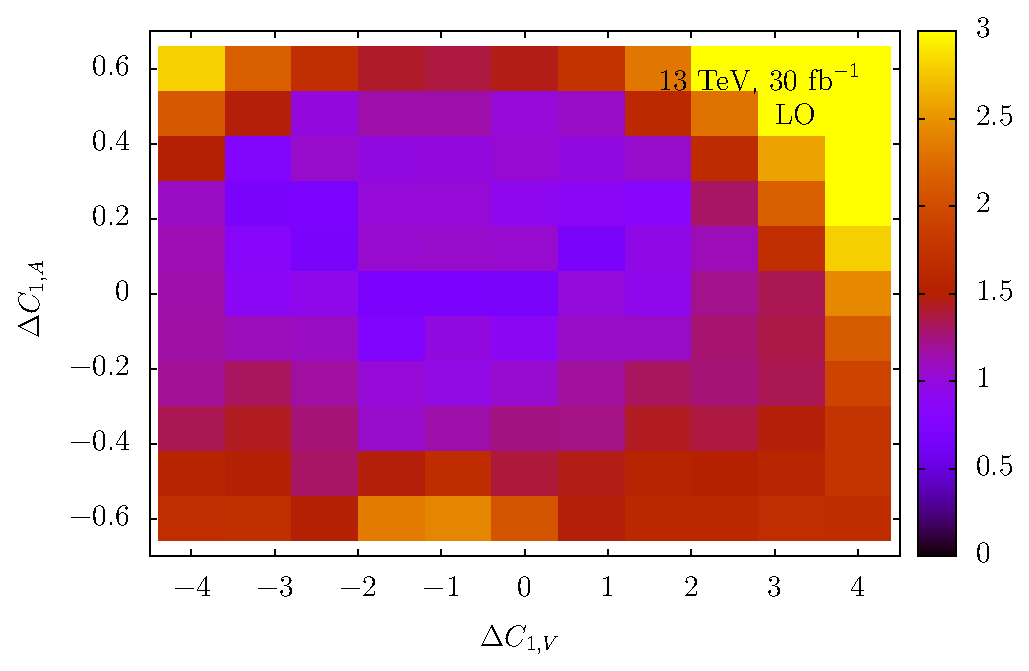
\includegraphics[scale=0.5]{LHC_53_LLSign_13LO30.eps} 
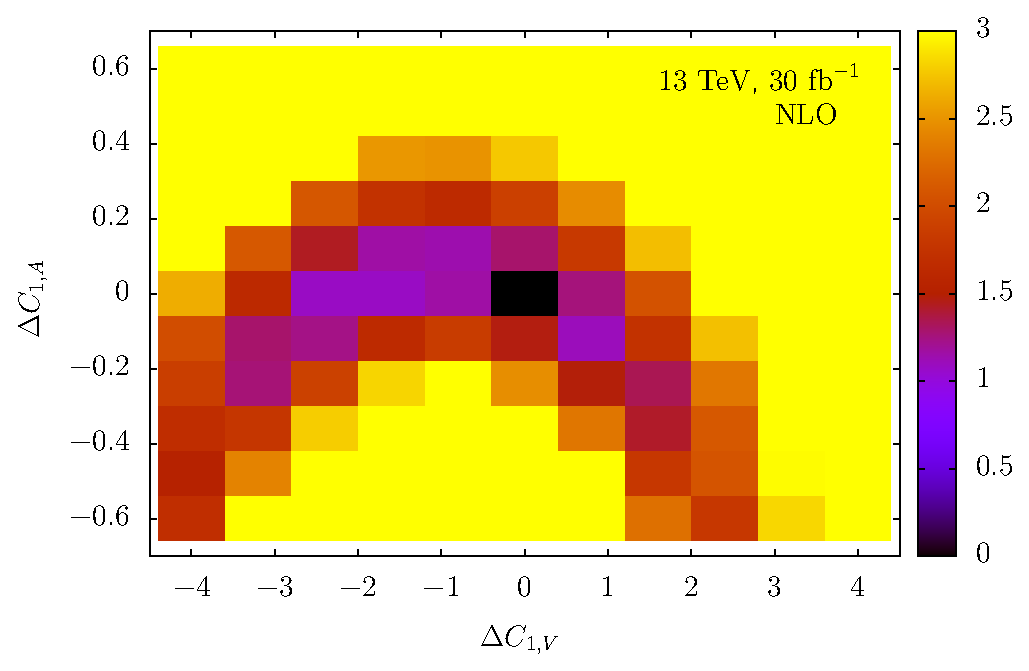
\includegraphics[scale=0.5]{LHC_53_LLSign_13NLO30.eps} 
\\
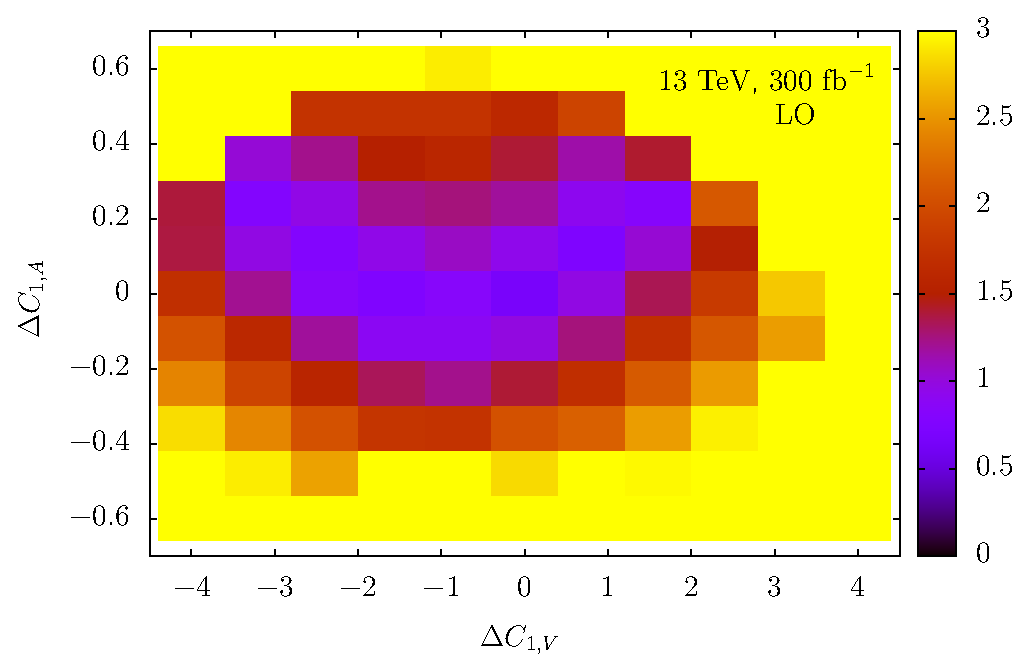
\includegraphics[scale=0.5]{LHC_53_LLSign_13LO300.eps} 
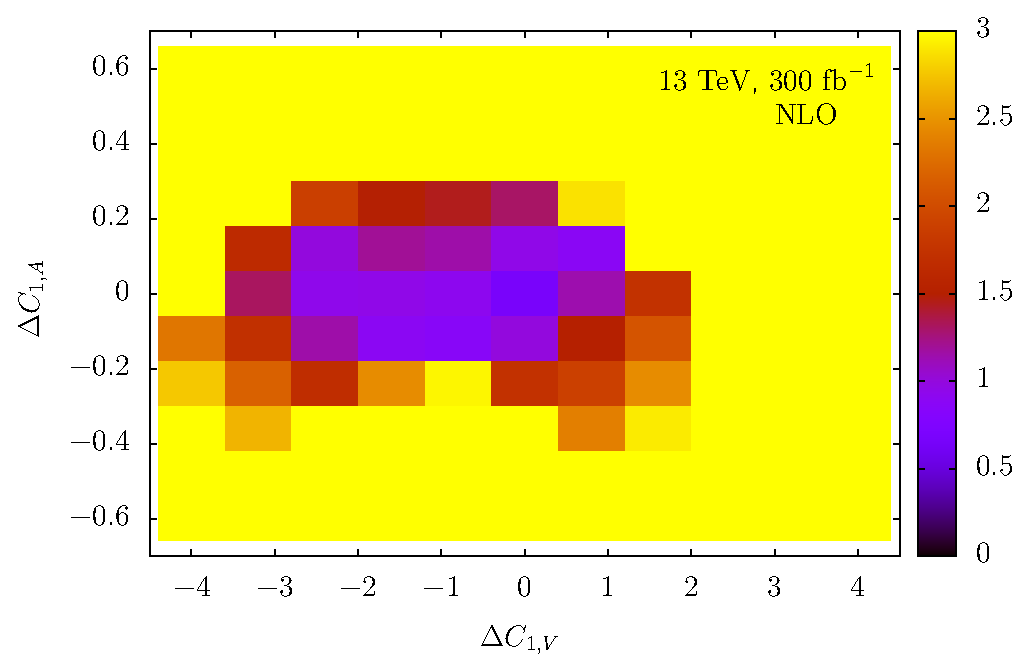
\includegraphics[scale=0.5]{LHC_53_LLSign_13NLO300.eps} 
\\
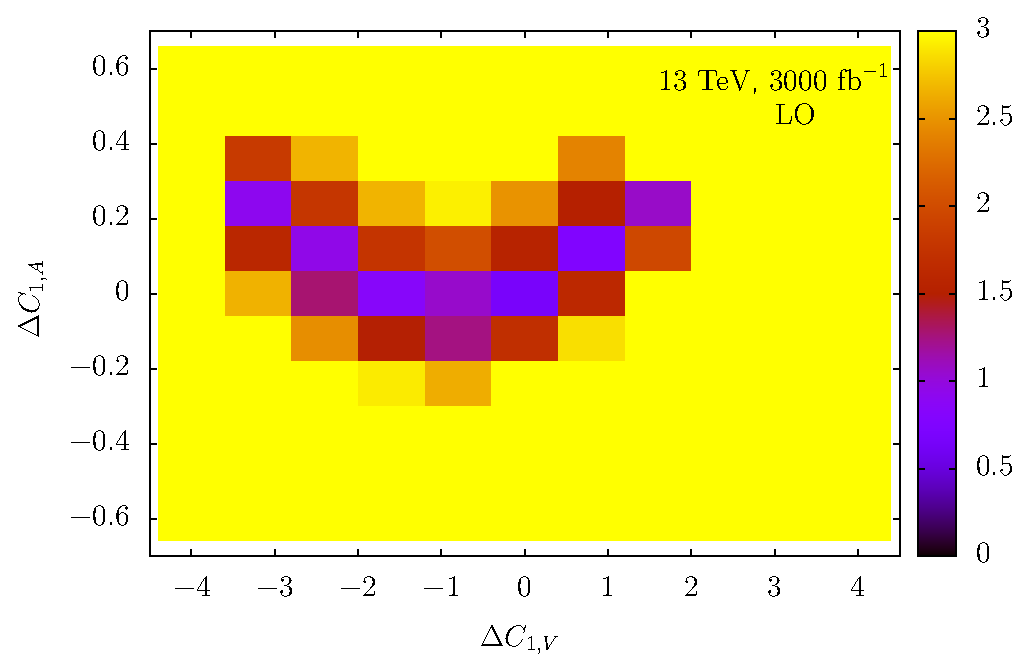
\includegraphics[scale=0.5]{LHC_53_LLSign_13LO3000.eps} 
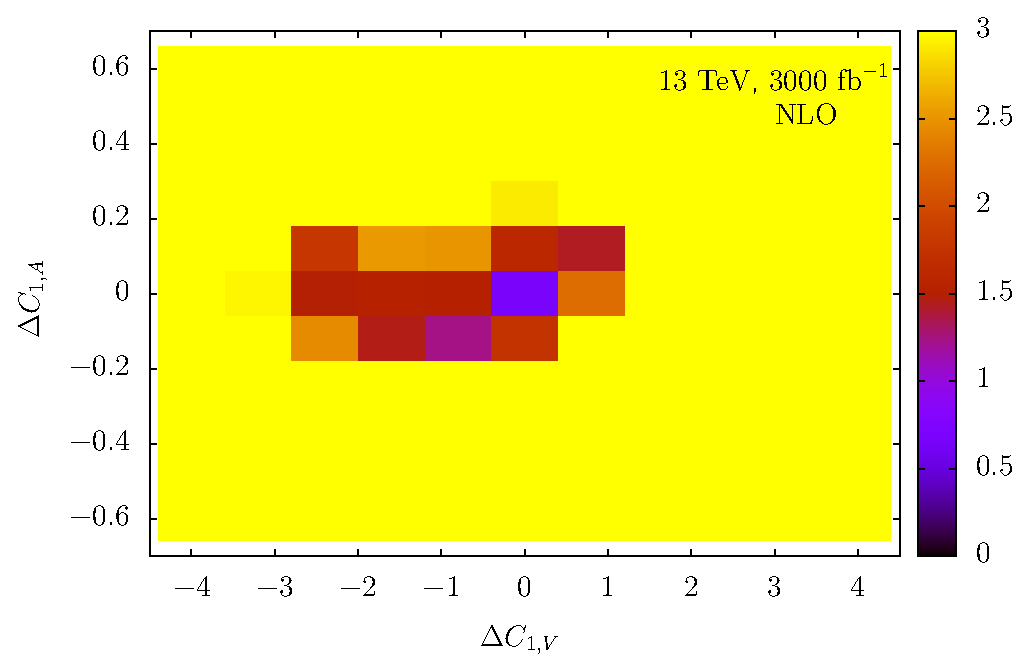
\includegraphics[scale=0.5]{LHC_53_LLSign_13NLO3000.eps} 
\caption{\label{fig:ix} Significance levels for deviations from SM vector and axial couplings $\DConeV$ and $\DConeA$,  using 30, 300 and 3000 $\invfb$ of data at the $\sqrt{s}=13$ TeV LHC. 
The results using LO results and uncertainties are shown on the left, results using NLO results and uncertainties are shown on the right.}
\end{figure}


The constraints are far stronger when NLO results and uncertainties are used, driven by the reduced uncertainty and a large $k$-factor of approximately 1.5. 
At this accuracy, the axial coupling can be constrained at $-0.2 \lesssim \DConeA \lesssim 0.15$ at the 1-$\sigma$ level and $-0.4 \lesssim \DConeA \lesssim 0.25$ 
at the 3-$\sigma$ level, independent of the value of $\ConeV$. Constraints on the vector coupling $\ConeV$ are still much looser: 
$-3 \lesssim \DConeV \lesssim 1.5$ at 1-$\sigma$ level and $-3 \lesssim \DConeV \lesssim 2.5$ at the 3-$\sigma$ level.

A feature of both of these plots which bears comment is the tongue of large $\sigma$ values which occurs for large values of $| \DConeV|$ and large 
negative values of $\DConeA$. This is best explained by considering the LO results for two points in the coupling parameter space, 
$(\DConeV,\DConeA)=(-0.40,+1.50)$ and $(\DConeV,\DConeA)=(-0.40,+2.00)$. These points lie 1.3 and 2.5 deviations from the SM hypothesis respectively; 
however, in the absence of theoretical uncertainties, the two hypotheses are 3.7 and 3.0 deviations away from the SM, respectively. 
The effect of introducing the uncertainties into the analysis is much more pronounced for the first point than for the second. 
The reason for this is that the main difference between the first point and the SM is the overall rate, whereas the second point has a similar rate to the 
SM but a significantly different shape (see fig.~\ref{fig:coupl_distr}). Then, for the second coupling choice, the values of $\nu_i^{\SM}$ and $\nu_i^{\alt}$ 
in each bin are similar, and the 
log of their ratio is small. The uncertainty enters the number of events $n_i$ in the bin, which is multiplied by this log. 
This means that the significance values are not greatly reduced by the theoretical uncertainty. 
The tongue of large $\sigma$-values therefore represents a set of points for which the distinction between the SM and alternate hypotheses 
is made based not on the overall rate, but rather on the shape of the $\Dphill$ distributions, which is relatively insensitive to the theoretical uncertainty. 
This also explains why the tongue is more prominent in the LO analysis.

%As can be seen in figure \ref{fig:coupl_distr}, there are significant shape changes for these values of the couplings, resulting in a large separation between the hypotheses. 
% At the same time, the overall rate is similar to the SM one.  
% The values of $\nu_i^{\SM}$ and $\nu_i^{\alt}$ in each bin are therefore similar, and the log of their ratio is small. 
% The uncertainty enters the number of events $n_i$ in the bin, which is multiplied by this log. 
% This means that the large significance values are not greatly reduced by the theoretical uncertainty.  
{\bf would this be seen in some other treatment of the scale uncertainty? corresponds to what you'd think, or not? on the one hand, 
the shape change should be less sensitive to the uncertainty than the overall cross-section. on the other, in each bin the number is similar to that of the SM, 
we should be able to wiggle them so that they coincide with the SM, whereas if the overall cross-section is very different from the SM, 
then the scale uncertainty can't do much. } 

In figure \ref{fig:LHC13data}, we show results of the analysis for 30 and 3000 $\invfb$ of data. 30 $\invfb$ of data should be available after 
the first year or so of the high energy run, while 3000 $\invfb$ is the benchmark value for the complete dataset over the lifetime of the LHC. 

%Dphill distr with LO and NLO scale bands, and two(three?) non-SM coupl\\
% $\sigma_{NP|} / \sigma_{SM}$ a la Berger, 0907.2191 \\

%Description of analysis Binned log likelihood, how we handle scale uncertainty (cf. Lykken et al) \\
% alpha plots - LO, NLO, rescaled (k-factor and reduced scale uncertainty) LO at 30, 300, 3000 fb-1\\
% Dphill distr normalized to $t\bar{t}$ cross-section  - 1 uncertainty from k-factors at 30, 300, 3000\\



\subsection{Limits on dimension-six operators}



Having presented our main results in Figs.~\ref{fig:CMS} and Figs.~\ref{fig:ix}, we can use the obtained limits to put constraints on 
possible effects of physics beyond the SM. 
The relevant dimension-6 operators have been presented in Sect.~\ref{sect:ttzcoupl}.
In this Section we also pointed out that the excellent agreement between experiment and prediction
for the $Z b_\mathrm{L} \bar{b}_\mathrm{L}$ coupling suggests $C^{(3,33)}_{\phi q} \approx - C^{(1,33)}_{\phi q}$.
In the following we will interpret this fact emperically and eliminate $C^{(1,33)}_{\phi q}$.
We begin by using the CMS cross section measurement at 7~TeV (see Sect.~\ref{sect:CMS}). 
The limits on the total $\ttbZ$ cross section as a function of $\DConeV$ and $\DConeA$ directly
translate into limits on the three operators in Eq.~\ref{EFTOp}. 
Diagonalizing the dependence in Eq.~\ref{Cone_NP}, we find at leading order
\be
 -15.7 \left(\frac{\Lambda}{1\,\mathrm{TeV}} \right)^2 
 \le  \mathrm{Re} \left[ C^{(3,33)}_{\phi q}  \right]   
 \le  21.1 \left(\frac{\Lambda}{1\,\mathrm{TeV}} \right)^2  ,
 \nonumber \\ \\ \nonumber 
 -50.2 \left(\frac{\Lambda}{1\,\mathrm{TeV}} \right)^2 
 \le  \mathrm{Re} \left[ C^{33}_{\phi u} \right]  
 \le 23.3 \left(\frac{\Lambda}{1\,\mathrm{TeV}} \right)^2. 
\ee
 Whereas using NLO input the limits improves to 
\be
 -13.4 \left(\frac{\Lambda}{1\,\mathrm{TeV}} \right)^2 
 \le  \mathrm{Re} \left[ C^{(3,33)}_{\phi q}  \right]   
 \le  20.0 \left(\frac{\Lambda}{1\,\mathrm{TeV}} \right)^2  ,
 \nonumber \\ \\ \nonumber
 -46.2 \left(\frac{\Lambda}{1\,\mathrm{TeV}} \right)^2 
 \le  \mathrm{Re} \left[ C^{33}_{\phi u} \right]  
 \le 18.9 \left(\frac{\Lambda}{1\,\mathrm{TeV}} \right)^2. 
\ee
Clearly this result should only be considered a first example for how constraints could be placed.
Meaningful limits are only obtained once more data is accumulated.
To estimate how limits will improve in such case, we use our results for the normalization and $\Delta \phi_{\ell\ell}$ shape 
analysis for the case of 30, 300, and 3000~$\invfb$.
For this case we find at leading order
\be
 \left. \begin{array}{l}
 xx \\
 -6.4 \\
 xx  
 \end{array} \right\}   \left(\frac{\Lambda}{1\,\mathrm{TeV}} \right)^2
 \le  \mathrm{Re} \left[ C^{(3,33)}_{\phi q} \right]  
 \le \left(\frac{\Lambda}{1\,\mathrm{TeV}} \right)^2  
 \left\{ \begin{array}{ll}
 yy & \quad 30  \, \invfb \\
 4.7 & \quad 300 \, \invfb \\
 yy & \quad 3000\, \invfb  
 \end{array} \right.
%  
 ,\nonumber \\  \\ \nonumber
%  
 \left. \begin{array}{l}
 xx \\
 -16.5 \\
 xx  
 \end{array} \right\} \left(\frac{\Lambda}{1\,\mathrm{TeV}} \right)^2
 \le  \mathrm{Re} \left[ C^{33}_{\phi u} \right]  
 \le yy \left(\frac{\Lambda}{1\,\mathrm{TeV}} \right)^2
 \left\{ \begin{array}{ll}
 yy & \quad 30  \, \invfb \\
 5.3 & \quad 300 \, \invfb \\
 yy & \quad 3000\, \invfb  
 \end{array} \right. .
\ee
At NLO QCD we find
\be
 \left. \begin{array}{l}
 xx \\
 -5.1 \\
 xx  
 \end{array} \right\}   \left(\frac{\Lambda}{1\,\mathrm{TeV}} \right)^2
 \le  \mathrm{Re} \left[ C^{(3,33)}_{\phi q}  \right]  
 \le \left(\frac{\Lambda}{1\,\mathrm{TeV}} \right)^2  
 \left\{ \begin{array}{ll}
 yy & \quad 30  \, \invfb \\
 2.7 & \quad 300 \, \invfb \\
 yy & \quad 3000\, \invfb  
 \end{array} \right.
%  
 ,\nonumber\\  \\\nonumber
%  
 \left. \begin{array}{l}
 xx \\
 -10.2 \\
 xx  
 \end{array} \right\} \left(\frac{\Lambda}{1\,\mathrm{TeV}} \right)^2
 \le  \mathrm{Re} \left[ C^{(33}_{\phi u} \right]  
 \le yy \left(\frac{\Lambda}{1\,\mathrm{TeV}} \right)^2
 \left\{ \begin{array}{ll}
 yy & \quad 30  \, \invfb \\
 3.4 & \quad 300 \, \invfb \\
 yy & \quad 3000\, \invfb  
 \end{array} \right. .
\ee
A graphical representaion of these limits, including their mutual dependence, is given in Fig.~\ref{fig:x} for $\Lambda=$1~TeV. 
We also include the indirect constraints from LEP measurements of $\varepsilon_1$ and $\varepsilon_b$.
As can be seen from the above results, something something...


\begin{figure}[t]
\centering
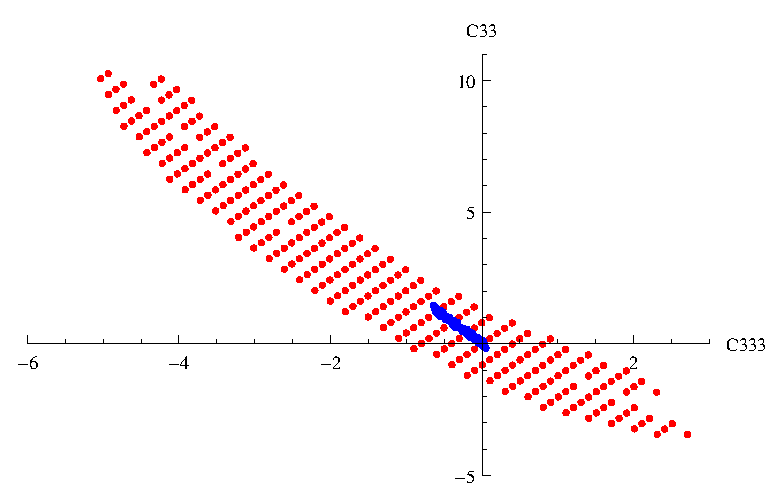
\includegraphics[scale=0.8]{OperatorLimits1TeVNLO.eps} 
\caption{\label{fig:x} Projected constraints on the operators $C^{(33,3)}_{\phi q}$ and $C^{33}_{\phi u}$}
\end{figure}


\section{Conclusion}
In this article we studied top quark pair production in association with a Z-boson.
Due to its relatively high production threshold and 
penalties from small branching fractions 
% small branching into a final state with two or more leptons 
this process was never observed at the Tevatron.
Even at the 7 and 8~TeV run of the LHC only a few candidate events were collected.
As a consequence there is no {\it direct} measurement of the top quark to Z-boson couplings to this date. 
This situation will change once the high energy LHC delievers its first 100~$\invfb$ of data.
We therefore study the process $pp\to\ttbZ$ at 13~TeV in the tri-lepton final state  
which provides the best compromise between clean signature and large enough cross section. 
We are particularly interested in answering the question by how much limits on
$\ttbZ$ couplings improve once NLO QCD predictions are used.
% Our theoretical description of production and decay dynamics is accurate to next-to-leading order QCD and
% accounts for all spin correlations at this order in perturbation theory. 
% Top quarks and the Z-boson are treated in the narrow-width approximation which is parameterically valid up to $\mathcal{O}(\Gamma \big/ m)$.
Our analysis for estimating the sensitivity to $\ttbZ$-couplings is preformed through a binned log-likelihood ratio test which is based on the 
distribution of the opening angle of the two leptons from the Z-boson decay.
To this end we generated a grid of $10^4$ different couplings and their corresponding kinematic distributions at NLO QCD. 
The results show that with 300~$\invfb$ the vector and axial couplings can be constrained to xx\% and yy\% accuracy at the 1-$\sigma$ C.L.
These limits are about yy times stronger compared to an analysis at leading order.
Our NLO QCD analysis also yields significant improvements on the limits when going from 300~$\invfb$ to 3000~$\invfb$.
This is not the case when leading order input is used due to large scale uncertainties.
% For the ultimate luminosity goal of 3000~$\invfb$ we find the limits xx\% and yy\% for vector and axial coupling, respectively.
We also translate our constraints on vector and axial couplings into limits on dimension-6 operators contributing to the $\ttbZ$ couplings beyond the SM.
We find that... but this cannot compete with indirect LEP constraints.

It would be an interesting future topic to study this sensitivity for an 100~TeV $pp$ collider or at an $e^+ e^-$ machine.
% This is mainly a result of the large residual scale dependence and large uncertainties from parton distribution functions at LO.
% We look forward to confronting our NLO QCD predictions with real data. 
Finally, we note that effects of New Physics can modify the $\ttbZ$-coupling beyond vector and axial currents through $q^2$-dependent  higher dimensional operators. 
Those couplings typically introduce non-renormalizable interactions and require an extension of the loop integrand reduction method. 
This is another interesting subject for a continuation of this work.
% other ideas: ttbar+large ETmiss (=Z->nunu)
%              e+ e- --> ttbar+2jets 
%              single top + Z
%              e+ e+ --> ttb z 
%              ttb + h , w, photon with anomalous couplings




\acknowledgments
We acknowledge helpful conversations with Y.~Gao, A.~Gritsan, N.~Tran and P.~Argrawal. 
Some of the numeric calculations weee done at NERSC.



\bibliographystyle{JHEP}
\bibliography{ttbZ}

\end{document}








